% Options for packages loaded elsewhere
\PassOptionsToPackage{unicode}{hyperref}
\PassOptionsToPackage{hyphens}{url}
%
\documentclass[
]{article}
\usepackage{lmodern}
\usepackage{amssymb,amsmath}
\usepackage{ifxetex,ifluatex}
\ifnum 0\ifxetex 1\fi\ifluatex 1\fi=0 % if pdftex
  \usepackage[T1]{fontenc}
  \usepackage[utf8]{inputenc}
  \usepackage{textcomp} % provide euro and other symbols
\else % if luatex or xetex
  \usepackage{unicode-math}
  \defaultfontfeatures{Scale=MatchLowercase}
  \defaultfontfeatures[\rmfamily]{Ligatures=TeX,Scale=1}
\fi
% Use upquote if available, for straight quotes in verbatim environments
\IfFileExists{upquote.sty}{\usepackage{upquote}}{}
\IfFileExists{microtype.sty}{% use microtype if available
  \usepackage[]{microtype}
  \UseMicrotypeSet[protrusion]{basicmath} % disable protrusion for tt fonts
}{}
\makeatletter
\@ifundefined{KOMAClassName}{% if non-KOMA class
  \IfFileExists{parskip.sty}{%
    \usepackage{parskip}
  }{% else
    \setlength{\parindent}{0pt}
    \setlength{\parskip}{6pt plus 2pt minus 1pt}}
}{% if KOMA class
  \KOMAoptions{parskip=half}}
\makeatother
\usepackage{xcolor}
\IfFileExists{xurl.sty}{\usepackage{xurl}}{} % add URL line breaks if available
\IfFileExists{bookmark.sty}{\usepackage{bookmark}}{\usepackage{hyperref}}
\hypersetup{
  pdftitle={Data Analysis for Public Affairs with R},
  pdfauthor={Jerome Dumortier},
  hidelinks,
  pdfcreator={LaTeX via pandoc}}
\urlstyle{same} % disable monospaced font for URLs
\usepackage[margin=1in]{geometry}
\usepackage{color}
\usepackage{fancyvrb}
\newcommand{\VerbBar}{|}
\newcommand{\VERB}{\Verb[commandchars=\\\{\}]}
\DefineVerbatimEnvironment{Highlighting}{Verbatim}{commandchars=\\\{\}}
% Add ',fontsize=\small' for more characters per line
\usepackage{framed}
\definecolor{shadecolor}{RGB}{248,248,248}
\newenvironment{Shaded}{\begin{snugshade}}{\end{snugshade}}
\newcommand{\AlertTok}[1]{\textcolor[rgb]{0.94,0.16,0.16}{#1}}
\newcommand{\AnnotationTok}[1]{\textcolor[rgb]{0.56,0.35,0.01}{\textbf{\textit{#1}}}}
\newcommand{\AttributeTok}[1]{\textcolor[rgb]{0.77,0.63,0.00}{#1}}
\newcommand{\BaseNTok}[1]{\textcolor[rgb]{0.00,0.00,0.81}{#1}}
\newcommand{\BuiltInTok}[1]{#1}
\newcommand{\CharTok}[1]{\textcolor[rgb]{0.31,0.60,0.02}{#1}}
\newcommand{\CommentTok}[1]{\textcolor[rgb]{0.56,0.35,0.01}{\textit{#1}}}
\newcommand{\CommentVarTok}[1]{\textcolor[rgb]{0.56,0.35,0.01}{\textbf{\textit{#1}}}}
\newcommand{\ConstantTok}[1]{\textcolor[rgb]{0.00,0.00,0.00}{#1}}
\newcommand{\ControlFlowTok}[1]{\textcolor[rgb]{0.13,0.29,0.53}{\textbf{#1}}}
\newcommand{\DataTypeTok}[1]{\textcolor[rgb]{0.13,0.29,0.53}{#1}}
\newcommand{\DecValTok}[1]{\textcolor[rgb]{0.00,0.00,0.81}{#1}}
\newcommand{\DocumentationTok}[1]{\textcolor[rgb]{0.56,0.35,0.01}{\textbf{\textit{#1}}}}
\newcommand{\ErrorTok}[1]{\textcolor[rgb]{0.64,0.00,0.00}{\textbf{#1}}}
\newcommand{\ExtensionTok}[1]{#1}
\newcommand{\FloatTok}[1]{\textcolor[rgb]{0.00,0.00,0.81}{#1}}
\newcommand{\FunctionTok}[1]{\textcolor[rgb]{0.00,0.00,0.00}{#1}}
\newcommand{\ImportTok}[1]{#1}
\newcommand{\InformationTok}[1]{\textcolor[rgb]{0.56,0.35,0.01}{\textbf{\textit{#1}}}}
\newcommand{\KeywordTok}[1]{\textcolor[rgb]{0.13,0.29,0.53}{\textbf{#1}}}
\newcommand{\NormalTok}[1]{#1}
\newcommand{\OperatorTok}[1]{\textcolor[rgb]{0.81,0.36,0.00}{\textbf{#1}}}
\newcommand{\OtherTok}[1]{\textcolor[rgb]{0.56,0.35,0.01}{#1}}
\newcommand{\PreprocessorTok}[1]{\textcolor[rgb]{0.56,0.35,0.01}{\textit{#1}}}
\newcommand{\RegionMarkerTok}[1]{#1}
\newcommand{\SpecialCharTok}[1]{\textcolor[rgb]{0.00,0.00,0.00}{#1}}
\newcommand{\SpecialStringTok}[1]{\textcolor[rgb]{0.31,0.60,0.02}{#1}}
\newcommand{\StringTok}[1]{\textcolor[rgb]{0.31,0.60,0.02}{#1}}
\newcommand{\VariableTok}[1]{\textcolor[rgb]{0.00,0.00,0.00}{#1}}
\newcommand{\VerbatimStringTok}[1]{\textcolor[rgb]{0.31,0.60,0.02}{#1}}
\newcommand{\WarningTok}[1]{\textcolor[rgb]{0.56,0.35,0.01}{\textbf{\textit{#1}}}}
\usepackage{longtable,booktabs}
% Correct order of tables after \paragraph or \subparagraph
\usepackage{etoolbox}
\makeatletter
\patchcmd\longtable{\par}{\if@noskipsec\mbox{}\fi\par}{}{}
\makeatother
% Allow footnotes in longtable head/foot
\IfFileExists{footnotehyper.sty}{\usepackage{footnotehyper}}{\usepackage{footnote}}
\makesavenoteenv{longtable}
\usepackage{graphicx,grffile}
\makeatletter
\def\maxwidth{\ifdim\Gin@nat@width>\linewidth\linewidth\else\Gin@nat@width\fi}
\def\maxheight{\ifdim\Gin@nat@height>\textheight\textheight\else\Gin@nat@height\fi}
\makeatother
% Scale images if necessary, so that they will not overflow the page
% margins by default, and it is still possible to overwrite the defaults
% using explicit options in \includegraphics[width, height, ...]{}
\setkeys{Gin}{width=\maxwidth,height=\maxheight,keepaspectratio}
% Set default figure placement to htbp
\makeatletter
\def\fps@figure{htbp}
\makeatother
\setlength{\emergencystretch}{3em} % prevent overfull lines
\providecommand{\tightlist}{%
  \setlength{\itemsep}{0pt}\setlength{\parskip}{0pt}}
\setcounter{secnumdepth}{5}

\title{Data Analysis for Public Affairs with R}
\author{Jerome Dumortier}
\date{2021-03-26}

\begin{document}
\maketitle

{
\setcounter{tocdepth}{2}
\tableofcontents
}
\hypertarget{preface}{%
\section{Preface}\label{preface}}

This book serves as an introduction to data analysis for public affairs with R and RStudio. Most examples are drawn from public affairs and economics. Throughout the book, the following notation is used

\begin{itemize}
\tightlist
\item
  \(variablename\): Variable names which represent the columns in a data frame.
\item
  \texttt{dataset}: Name of the data set in the file \texttt{DataAnalysisPAData.RData}.
\item
  \emph{Exercise Name}: Title of the exercise in the various chapters.
\item
  \href{https://cran.r-project.org/web/packages/plm/index.html}{package}: Link to the package documents. The link presented is associated with ``Linear Models for Panel Data.''
\end{itemize}

\hypertarget{introduction}{%
\section{Introduction}\label{introduction}}

\hypertarget{introduction-to-r}{%
\section{Introduction to R}\label{introduction-to-r}}

Topics covered in this lecture

\begin{itemize}
\tightlist
\item
  Introduction to R and RStudio
\item
  Data Management
\item
  Plotting and Graphs with R
\item
  Basic Statistics
\end{itemize}

In-class exercises will be conducted throughout the Lecture.

\hypertarget{online-resources-and-help}{%
\subsection{Online Resources and Help}\label{online-resources-and-help}}

Very large user community for R. Google search for ``Some topic R'' usually leads quickly to the desired help.
Here are the links to a few online tutorials

\begin{itemize}
\tightlist
\item
  \href{http://stats.idre.ucla.edu/r/}{UCLA Institute for Digital Research and Education}
\item
  \href{https://www.statmethods.net/}{StatMethods}
\item
  \href{http://www.sthda.com/english/}{Statistical tools for high-throughput data analysis}
\end{itemize}

Two online resources will provide you the solution to the vast majority of your R questions. Getting on those websites is usually the result of a Google search.

\begin{itemize}
\tightlist
\item
  \href{https://stat.ethz.ch/R-manual/}{Statistical Data Analysis R}: This resource contains the function manual for R/RStudio including all packages. Example for a function \href{https://stat.ethz.ch/R-manual/R-devel/library/graphics/html/boxplot.html}{boxplot}. The most helpful part are the examples at the bottom of the page.
\item
  Stack Overflow: Resources for developers. For example, a Google search for ``r ggplot two y axis'' may give you the following \href{https://stackoverflow.com/questions/3099219/plot-with-2-y-axes-one-y-axis-on-the-left-and-another-y-axis-on-the-right}{result} Note that all questions on Stack Overflow have to be accompanied by a re-creatable dataset.
\end{itemize}

Besides many online resources, there are also two useful textbooks

\begin{itemize}
\tightlist
\item
  \href{https://link.springer.com/book/10.1007/978-0-387-77318-6}{Applied Econometrics with R} by Christian Kleiber and Achim Zeileis.
\item
  \href{https://link.springer.com/book/10.1007/978-0-387-79054-1\%5D}{Introductory Statistics with R} by Peter Dalgaard.
\end{itemize}

An additional online tutorial is \href{https://cran.r-project.org/doc/contrib/Verzani-SimpleR.pdf\%5D}{Using R for Introductory Statistics} by John Verzani.

\hypertarget{opening-rstudio}{%
\subsection{Opening RStudio}\label{opening-rstudio}}

Work in RStudio is done in four windows:

\begin{enumerate}
\def\labelenumi{\arabic{enumi}.}
\tightlist
\item
  Script Window

  \begin{itemize}
  \tightlist
  \item
    This is were you type your R Script (.R) and where you execute commands.
  \item
    Comparable to do-file/editor in Stata.
  \item
    This window needs to be opened by File \(\Rightarrow\) New File \(\Rightarrow\) R Script.
  \end{itemize}
\item
  Console window

  \begin{itemize}
  \tightlist
  \item
    Use of R interactively. Should only be used for quick calculations and not part of an analysis.
  \end{itemize}
\item
  Environment

  \begin{itemize}
  \tightlist
  \item
    Lists all the variables, data frames, and user-created functions.
  \item
    It is tempting to use the ``Import Dataset'' function \dots Don't.
  \end{itemize}
\item
  Plots/Packages/Help
\end{enumerate}

There is a base version of R that allows doing many calculations but the power of R comes through its packages. To use functions associated with a particular package, click ``Install'' in the packages window of RStudio and type in the name of the package. Or alternatively, use

\begin{itemize}
\tightlist
\item
  \texttt{install.packages("ggplot2")}
\end{itemize}

To use a package, you have to activate it by either checking the box in the window ``Packages'' or by including \texttt{library(packagename)}. Those packages are updated on a regular basis by users.

The \texttt{\textbackslash{}\#} allows you to include comments in your script file that are not read by R. It is good practice to start any new script with clearing the memory using the command \texttt{rm(list=ls())}. Use the command \texttt{get()} to determine the current working directory or set the new working directory with the command \texttt{setwd()}, e.g., \texttt{setwd("E:/")}. For file paths, replace \(\backslash\) with \(/\). Next, you want to load all libraries necessary for your entire script file with the command \texttt{library()}. It is also good practice to save your R-script on a regular basis. The frontmatter, i.e., the top of a R-script file, could look as follows

\begin{Shaded}
\begin{Highlighting}[]
\KeywordTok{rm}\NormalTok{(}\DataTypeTok{list=}\KeywordTok{ls}\NormalTok{())}
\KeywordTok{load}\NormalTok{(}\StringTok{"DataAnalysisPAData.RData"}\NormalTok{)}
\KeywordTok{library}\NormalTok{(openxlsx)}
\end{Highlighting}
\end{Shaded}

\hypertarget{in-class-exercise-1}{%
\subsubsection{In-class Exercise 1}\label{in-class-exercise-1}}

Create a R-script file with the following components:

\begin{enumerate}
\def\labelenumi{\arabic{enumi}.}
\tightlist
\item
  Two lines for the title and the date (use \#)
\item
  Clearing all current contents
\item
  Setting the correct working directory

  \begin{itemize}
  \tightlist
  \item
    This should be a folder to which you have downloaded all materials.
  \end{itemize}
\item
  Installing and loading the package \texttt{openxlsx}.
\end{enumerate}

\hypertarget{functions}{%
\subsection{Functions}\label{functions}}

At the core of R are functions that ``do things'' based on your input. The basic structure is

\begin{itemize}
\tightlist
\item
  \texttt{object\ =\ functionname(argument1=value,argument2=value,...)}
\end{itemize}

The structure has the following components

\begin{itemize}
\tightlist
\item
  \texttt{object}: Output of the function will be assigned to object.
\item
  \texttt{functionname}: Name of the system function. You can also create and use your own functions. More about this later.
\item
  \texttt{argument}: Arguments are function specific.
\item
  \texttt{value}: The value you want a particular argument to take.
\end{itemize}

If a function is executed without an specific assignment, the output will be displayed in the console window. Before using a function, read the documentation. Many functions have default settings. Be aware of default values. In most cases, those defaults are set to values that satisfy most uses. For example, consider the help file for the function \href{https://stat.ethz.ch/R-manual/R-devel/library/stats/html/t.test.html}{t.test}.

-\texttt{t.test(x,y=NULL,...,mu=0,conf.level=0.95,...)}

For this function we have the following default values

\begin{itemize}
\tightlist
\item
  \texttt{y=NULL}
\item
  \texttt{mu=0}
\item
  \texttt{conf.level=0.95}
\end{itemize}

\hypertarget{data-management}{%
\subsection{Data Management}\label{data-management}}

\hypertarget{data-in-r}{%
\subsubsection{Data in R}\label{data-in-r}}

The main data types which can appear in the Environment window of R are:

\begin{itemize}
\tightlist
\item
  Vectors

  \begin{itemize}
  \tightlist
  \item
    \texttt{preselection\ =\ seq(1788,2016,4)}
  \item
    \texttt{midterm\ =\ seq(by=4,to=2018,from=1790)}
  \end{itemize}
\item
  Matrix

  \begin{itemize}
  \tightlist
  \item
    \texttt{somematrix\ =\ matrix(8,10,4)}
  \item
    Only numerical values are allowed.
  \end{itemize}
\item
  Data frames

  \begin{itemize}
  \tightlist
  \item
    By far, the most common data type in R.
  \item
    Comparable to an Excel sheet.
  \item
    More on this later.
  \end{itemize}
\item
  Lists

  \begin{itemize}
  \tightlist
  \item
    Collection of objects from of various types.
  \item
    \texttt{myfirstlist\ =\ list(preselection,midterm,somematrix)}
  \end{itemize}
\end{itemize}

\hypertarget{using-r-as-a-calculator}{%
\subsubsection{Using R as a Calculator}\label{using-r-as-a-calculator}}

Entering heights of people and storing it in a vector named \emph{height}:

\begin{Shaded}
\begin{Highlighting}[]
\NormalTok{height =}\StringTok{ }\KeywordTok{c}\NormalTok{(}\DecValTok{71}\NormalTok{,}\DecValTok{77}\NormalTok{,}\DecValTok{70}\NormalTok{,}\DecValTok{73}\NormalTok{,}\DecValTok{66}\NormalTok{,}\DecValTok{69}\NormalTok{,}\DecValTok{73}\NormalTok{,}\DecValTok{73}\NormalTok{,}\DecValTok{75}\NormalTok{,}\DecValTok{76}\NormalTok{)}
\end{Highlighting}
\end{Shaded}

Calculating the sum, product, natural log, mean, and (element-wise) squaring is done with the following commands:

\begin{itemize}
\tightlist
\item
  \texttt{sum(height)}
\item
  \texttt{prod(height)}
\item
  \texttt{log(height)} \# Default is the natural log
\item
  \texttt{meanheight\ =\ mean(height)}
\item
  \texttt{heightsq\ =\ height\^{}2}
\end{itemize}

Removing (i.e., deleting) unused elements: \texttt{rm(heightsq,meanheight)}

\hypertarget{creating-a-data-frame-from-scratch}{%
\subsubsection{Creating a Data Frame from Scratch}\label{creating-a-data-frame-from-scratch}}

Data frames are the most commonly used tables in R/RStudio. They are similar to an Excel sheet.

\begin{itemize}
\tightlist
\item
  Column names represent the variables and rows represent observations.
\item
  Column names must be unique and without spaces.
\end{itemize}

Suggestion: Use only lower-case variable names and objects.

\begin{Shaded}
\begin{Highlighting}[]
\NormalTok{studentid       =}\StringTok{ }\DecValTok{1}\OperatorTok{:}\DecValTok{10}
\NormalTok{studentnames    =}\StringTok{ }\KeywordTok{c}\NormalTok{(}\StringTok{"Andrew"}\NormalTok{,}\StringTok{"Linda"}\NormalTok{,}\StringTok{"William"}\NormalTok{,}\StringTok{"Daniel"}\NormalTok{,}\StringTok{"Gina"}\NormalTok{,}
                    \StringTok{"Mick"}\NormalTok{,}\StringTok{"Sonny"}\NormalTok{,}\StringTok{"Wilbur"}\NormalTok{,}\StringTok{"Elisabeth"}\NormalTok{,}\StringTok{"James"}\NormalTok{)}
\NormalTok{students        =}\StringTok{ }\KeywordTok{data.frame}\NormalTok{(studentid,studentnames,height)}
\KeywordTok{rm}\NormalTok{(studentid,height,studentnames)}
\end{Highlighting}
\end{Shaded}

\hypertarget{in-class-exercise-2}{%
\subsubsection{In-class Exercise 2}\label{in-class-exercise-2}}

Create a data frame called \texttt{students} containing the following information:

\begin{tabular}{l|r|r}
\hline
Name & Economics & English\\
\hline
Mindy & 80.0 & 52.5\\
\hline
Gregory & 60.0 & 60.0\\
\hline
Shubra & 95.0 & 77.5\\
\hline
Keith & 77.5 & 30.0\\
\hline
Louisa & 97.5 & 95.0\\
\hline
\end{tabular}

Notes:

\begin{itemize}
\tightlist
\item
  Use \emph{name} as the column header for the students' names.
\item
  Once you have created the data frame, remove the unused vectors.
\end{itemize}

\hypertarget{basic-multivariate-regression}{%
\section{Basic Multivariate Regression}\label{basic-multivariate-regression}}

Extension of the bivariate model to multivariate regression

\begin{itemize}
\tightlist
\item
  One dependent variable but multiple independent variables
\end{itemize}

Topics associated with multivariate regression models covered in this lecture:

\begin{itemize}
\tightlist
\item
  Multicollinearity
\item
  Dummy Variables
\item
  Natural logarithm
\item
  Functional forms
\item
  Interaction Terms
\end{itemize}

Bivariate regression model (one independent and one dependent variable)
\begin{equation*}
            y = \beta_0 + \beta_1 x_1 + \epsilon
        \end{equation*}
Multivariate linear regression model (multiple independent variables)
\begin{equation*}
            y = \beta_0 + \beta_1 x_1 + \beta_2 x_2 + \dots + \beta_k x_k + \epsilon
        \end{equation*}
Whether we consider the univariate or multivariate regression model, the objective is always to minimize the sum of squared errors, hence the name ordinary least square (OLS) model. The equation of a line can be determined using slope and intercept, we can write:
\begin{equation*}
            E(y|x) = \beta_0 + \beta_1 x
        \end{equation*}
A model with two independent variables (predictors) describes a plane.

\hypertarget{dummy-variables}{%
\subsection{Dummy Variables}\label{dummy-variables}}

Dummy variables represent a single qualitative characteristic such as religion, gender, or nationality. Dummy variables are independent variables coded as either 0 or 1. For example, consider

Example: Price (\(Y_i\)) of a car depending on miles (\(X_i\)) and AWD (\(D_i\))
\begin{equation*}
                    Y_i = \beta_0 + \beta_1 X_i + \beta_2 D_i + \epsilon_i
                \end{equation*}
with \(D_i = 1\) if AWD and \(D_i = 0\) if RWD.
\textbackslash end\{itemize\}
This regression can theoretically be separated into two single equations:

\begin{enumerate}
            \item RWD: $Y_i = \beta_0 + \beta_1 X_i + \epsilon_i$
            \item AWD: $Y_i = (\beta_0 + \beta_2 )+ \beta_1 X_i + \epsilon_i$
        \end{enumerate}

Interpretation:

\begin{itemize}
            \item Knowledge on how the dummy-variable was coded.
            \item If the coefficient of the dummy-variable ``adds'' (or ``subtracts'' if sign is negative) compared to the 0-group.
        \end{itemize}

\hypertarget{anova}{%
\section{ANOVA}\label{anova}}

Analysis of Variance (ANOVA) models (also know as Dummy Variable Regression models) are regressions with only dummy variables. An ANOVA model with two independent variables can be written as follows:
\[y_i = \beta_0 + \beta_1 \cdot d_1 + \beta_2 \cdot d_2\]
where \(d_1\) and \(d_2\) are dummy variables. Consider the following model using the \texttt{gss2018} data:
\[income = \beta_0 + \beta_1 \cdot fulltime + \beta_2 \cdot government\]
where \emph{fulltime} and \emph{government} are dummy variables. That is, if \(fulltime=1\), then the person has a fulltime job. If \(government=1\), then the respondent works for the government. To distinguish \emph{j} categories only \emph{j-1} dummy variables are needed. Otherwise, we have perfect multicollinearity. The category without a dummy variable is the base category.

\begin{Shaded}
\begin{Highlighting}[]
\NormalTok{bhat =}\StringTok{ }\KeywordTok{lm}\NormalTok{(income}\OperatorTok{~}\NormalTok{fulltime}\OperatorTok{+}\NormalTok{government,}\DataTypeTok{data=}\NormalTok{gss2018)}
\KeywordTok{summary}\NormalTok{(bhat)}
\end{Highlighting}
\end{Shaded}

\begin{verbatim}
## 
## Call:
## lm(formula = income ~ fulltime + government, data = gss2018)
## 
## Residuals:
##    Min     1Q Median     3Q    Max 
## -51074 -23574  -6074  16426 152479 
## 
## Coefficients:
##             Estimate Std. Error t value Pr(>|t|)    
## (Intercept)    17521       3377   5.189 2.71e-07 ***
## fulltime       33553       3691   9.091  < 2e-16 ***
## government     -6840       3640  -1.879   0.0606 .  
## ---
## Signif. codes:  0 '***' 0.001 '**' 0.01 '*' 0.05 '.' 0.1 ' ' 1
## 
## Residual standard error: 39230 on 769 degrees of freedom
## Multiple R-squared:  0.099,  Adjusted R-squared:  0.09665 
## F-statistic: 42.25 on 2 and 769 DF,  p-value: < 2.2e-16
\end{verbatim}

The income for a person who is working neither for the government nor has a full time job makes on average \$17,521. A person not working for the government but with a full time job is earning \$17,521+\$33,553=\$51,074. Note that both dummy variables are statistically significant. Note that the R-squared is very low.

\hypertarget{exercises}{%
\subsection{Exercises}\label{exercises}}

\begin{enumerate}
\def\labelenumi{\arabic{enumi}.}
\tightlist
\item
  Consider the data in \texttt{indyhomes}. A real estate agent once mentioned that homes built in the eighties are of lower quality and thus, are cheaper. One possibility to asses this claim is with an ANOVA model. Add three new dummy variables to the data frame: eighties (equal to 1 if the home was built in any year between 1980 to 1989), northwest (equal to 1 if the home is in the 46268 ZIP code), and singlestory (equal to 1 if the home has one story). Estimate the following ANOVA model:
  \[price = \beta_0+\beta_1 \cdot d_{80s}+\beta_2 \cdot d_{northwest} + \beta_3 \cdot d_{single}\]
  What do you conclude? Next, add square footage to the model. What has changed in terms of coefficicents? How do you interpret that change?
\end{enumerate}

\hypertarget{violating-assumptions}{%
\section{Violating Assumptions}\label{violating-assumptions}}

This chapter introduces the detection and correction of problems with the estimation procedure due to the violation of the key assumptions necessary for the OLS model to work. The following R packages are needed for this chapter: \texttt{car}, \texttt{lmtest}, \texttt{orcutt}, and \texttt{sandwich}.

\hypertarget{heteroscedasticity}{%
\subsection{Heteroscedasticity}\label{heteroscedasticity}}

A key assumption of the OLS model is homoscedasticity error terms. That is, the error variance is constant:
\[Var(\epsilon_i) = \sigma^2\]
With heteroscedasticity, the variance of the error term is not constant:
\[Var(\epsilon_i) = \sigma_i^2\]
For a bivariate regression model with heteroscedastic data, it can be shown that
\[Var(\hat{\beta_1}) = \frac{\sum x_i^2 \sigma_i^2}{(\sum x_i^2)^2}\]
This is different from the variance of the coefficient estimate under homoscedasticity:
\[Var(\hat{\beta_1}) = \frac{\sigma^2}{\sum x_i^2}\]
Unbiasedness of the OLS estimator is not affected but the variance of \(\beta_1\) will be larger compared to other estimators. Note that the measure of \(R^2\) is unaffected by heteroscedasticity. Homoscedasticity is needed to justify the t-test, F-test, and confidence intervals. The F-statistic does no longer have an F-distribution. In short, hypothesis tests on the \(\beta\)-coefficients are no longer valid.

If \(\sigma_i^2\) was known, the use of a Generalized Least Squares (GLS) model would be appropriate:
\[y_i = \beta_0 + \beta_1 \cdot x_i + \epsilon_i\]
Dividing both sides by the known variance:
\[\frac{y_i}{\sigma_i}=\beta_0 \cdot \frac{1}{\sigma_i}+\beta_1 \frac{x_i}{\sigma_i}+\frac{\epsilon_i}{\sigma_i}\]
If \(\epsilon^*_i = \epsilon_i / \sigma_i\), then it can be shown that \(Var(\epsilon^*_i)=1\), i.e., constant. Under the usual OLS model:
\[\sum_{i=1}^N e_i^2=\sum_{i=1}^N \left(y_i-\hat{\beta}_0+\hat{\beta}_1 \cdot x_i \right)^2\]
Under GLS model:
\[\sum_{i=1}^N w_i e_i^2= \sum_{i=1}^N w_i \left(y_i-\hat{\beta}_0+\hat{\beta}_1 \cdot x_i \right)^2\]
That is, GLS minimizes the weighted sum of the residual squares. Since in reality, the variance of \(\sigma^2\) is not known, other techniques have to be employed to obtain so-called heteroscedasticity-consistent (HC) standard errors. But first, two tests are introduced to detect heteroscedasticity.

\hypertarget{detecting-heteroscedasticity}{%
\subsubsection{Detecting Heteroscedasticity}\label{detecting-heteroscedasticity}}

Two test are presented to detect heteroscedasticity:

\begin{itemize}
\tightlist
\item
  Goldfeld-Quandt Test (1965)
\item
  Breusch-Pagan-Godfrey Test (1979)
\end{itemize}

The steps necessary for the \textbf{Goldfeld-Quandt Test} are as follows:

\begin{enumerate}
\def\labelenumi{\arabic{enumi}.}
\tightlist
\item
  Sort observations by ascending order of the dependent variable.
\item
  Pick \emph{C} as the number of central observations to drop in the middle of the dependent variable.
\item
  Run two separate regression equations, i.e., with the ``lower'' and ``upper'' part.
\item
  Compute
  \[\lambda = \frac{RSS_2/df}{RSS_1/df}\]
\item
  \(\lambda\) follows an F-distribution.
\end{enumerate}

The Goldfeld-Quandt Test can be illustrated with \texttt{gqtestdata}. In a first step, the data is separated into two groups with \(C=6\). In a second step, both groups are used to run a regression. And lastly, \(\lambda\) is calculated.

\begin{Shaded}
\begin{Highlighting}[]
\NormalTok{gqtestdata1         =}\StringTok{ }\NormalTok{gqtestdata[}\DecValTok{1}\OperatorTok{:}\DecValTok{22}\NormalTok{,]}
\NormalTok{gqtestdata2         =}\StringTok{ }\NormalTok{gqtestdata[}\DecValTok{29}\OperatorTok{:}\DecValTok{50}\NormalTok{,]}
\NormalTok{bhat1               =}\StringTok{ }\KeywordTok{lm}\NormalTok{(price_r}\OperatorTok{~}\NormalTok{sqft_r,}\DataTypeTok{data=}\NormalTok{gqtestdata1)}
\NormalTok{bhat2               =}\StringTok{ }\KeywordTok{lm}\NormalTok{(price_r}\OperatorTok{~}\NormalTok{sqft_r,}\DataTypeTok{data=}\NormalTok{gqtestdata2)}
\NormalTok{lambda              =}\StringTok{ }\KeywordTok{sum}\NormalTok{(bhat2}\OperatorTok{$}\NormalTok{residuals}\OperatorTok{^}\DecValTok{2}\NormalTok{)}\OperatorTok{/}\KeywordTok{sum}\NormalTok{(bhat1}\OperatorTok{$}\NormalTok{residuals}\OperatorTok{^}\DecValTok{2}\NormalTok{)}
\end{Highlighting}
\end{Shaded}

Of course, there is also a function in R called gqtest which simplifies the procedure.

\begin{Shaded}
\begin{Highlighting}[]
\KeywordTok{library}\NormalTok{(lmtest)}
\NormalTok{bhat                =}\StringTok{ }\KeywordTok{lm}\NormalTok{(price}\OperatorTok{~}\NormalTok{sqft,}\DataTypeTok{data=}\NormalTok{gqtestdata)}
\KeywordTok{gqtest}\NormalTok{(bhat,}\DataTypeTok{fraction =} \DecValTok{6}\NormalTok{)}
\end{Highlighting}
\end{Shaded}

\begin{verbatim}
## 
##  Goldfeld-Quandt test
## 
## data:  bhat
## GQ = 6.7361, df1 = 20, df2 = 20, p-value = 3.928e-05
## alternative hypothesis: variance increases from segment 1 to 2
\end{verbatim}

In any case, the hypothesis of homoscedasticity is rejected for \texttt{gqtestdata}.

The \textbf{Breusch-Pagan-Godfrey Test} is an alternative and does not rely on choosing \emph{C} as the number of central observations to be dropped. The steps include the following:

\begin{enumerate}
\def\labelenumi{\arabic{enumi}.}
\tightlist
\item
  Run a regular OLS model and obtain the residuals.
\item
  Calculate
  \[\hat{\sigma}^2 = \frac{\sum_{i=1}^N e^2_i}{N}\]
\item
  Construct the variable \(p_i\) as follows: \(p_i = e^2_i / \hat{\sigma}^2\)
\item
  Regress \(p_i\) on the X's as follows
  \[p_i = \alpha_0 + \alpha_1 \cdot x_{i1}+\alpha_2 \cdot x_{i2} + \dots\]
\item
  Obtain the explained sum of squares (ESS) and define \(\Theta = 0.5 \cdot ESS\). Then \(\Theta \sim \chi^2_{m-1}\).
\end{enumerate}

The much simpler procedure is to use the function \texttt{bptest()} in R.

\begin{Shaded}
\begin{Highlighting}[]
\KeywordTok{library}\NormalTok{(lmtest)}
\NormalTok{bhat                =}\StringTok{ }\KeywordTok{lm}\NormalTok{(price}\OperatorTok{~}\NormalTok{sqft,}\DataTypeTok{data=}\NormalTok{gqtestdata)}
\KeywordTok{bptest}\NormalTok{(bhat)}
\end{Highlighting}
\end{Shaded}

\begin{verbatim}
## 
##  studentized Breusch-Pagan test
## 
## data:  bhat
## BP = 15.01, df = 1, p-value = 0.0001069
\end{verbatim}

\hypertarget{correcting-heteroscedasticity}{%
\subsubsection{Correcting Heteroscedasticity}\label{correcting-heteroscedasticity}}

To correct for heteroscedasticity, robust standard errors must be obtained.

\begin{Shaded}
\begin{Highlighting}[]
\KeywordTok{library}\NormalTok{(sandwich)}
\NormalTok{bhat =}\StringTok{ }\KeywordTok{lm}\NormalTok{(price}\OperatorTok{~}\NormalTok{sqft,}\DataTypeTok{data=}\NormalTok{gqtestdata)}
\KeywordTok{summary}\NormalTok{(bhat)}
\NormalTok{vcov =}\StringTok{ }\KeywordTok{vcovHC}\NormalTok{(bhat)}
\KeywordTok{coeftest}\NormalTok{(bhat,}\DataTypeTok{vcov.=}\NormalTok{vcov)}
\end{Highlighting}
\end{Shaded}

Note that there are multiple variations to calculate the standard error and thus, it is possible for slight variations among the results from different packages.
\[Var(\hat{\beta}_1) = \frac{\sum_{i=1}^N (x_i-\bar{x})^2 e_i^2}{\sum_{i=1}^N (x_i-\bar{x})^2}\]
The square root of the following equation is called heteroscedastic robust standard error:
\[\widehat{Var}(\hat{\beta}_j) = \frac{\sum_{i=1}^N \hat{r}^2_{ij} e_i^2}{\sum_{i=1}^N (x_i-\bar{x})^2}\]
Standard errors can be either larger or smaller. Note that in this example, we do not know whether heteroscedasticity is present or not.

\hypertarget{multicollinearity}{%
\subsection{Multicollinearity}\label{multicollinearity}}

Multicollinearity describes the situation in which two or more independent variables are linearly related. Under perfect multicollinearity:
\[\lambda_1 x_1 + \lambda_2 x_2 + \dots +\lambda_k x_k = 0\]
where \(\lambda_i\) are constants that are not all zero simultaneously. For example, consider \(x_1=\{8,12,15,17\}\), \(x_2=\{24,36,45,51\}\), and \(x_3=\{2,3,3.75,4.25\}\). In this case, \(\lambda_1=1\), \(\lambda_2=-1/5\), and \(\lambda_3=2\). Note, multicollinearity refers to linear relationships! Including a squared or cubed term is not an issue of multicollinearity. It can be shown that the variance of the estimator increases in the presence of multicollinearity. There are various indications that the data suffers from multicollinearity:

\begin{itemize}
\tightlist
\item
  High \(R^2\) but few significant variables
\item
  Fail to reject the hypothesis for H\(_0\): \(\beta_i=0\) based on t-values but rejection all slopes being simultaneously zero based on F-test.
\item
  High correlation among explanatory variables
\item
  Variation of statistically significant variables between models.
\end{itemize}

\hypertarget{variance-inflated-factors-vif}{%
\subsubsection{Variance Inflated Factors (VIF)}\label{variance-inflated-factors-vif}}

Identifies possible correlation among multiple independent variables and not just two as in the case of a simple correlation coefficient. Consider the model:
\[y_i = \beta_0 + \beta_k x_{ik} + \epsilon_i\]
The estimated variances of the coefficient \(\beta_k\) is written as
\[Var(\beta_k)^* = \frac{\sigma^2}{\sum_{i=1}^N (x_{ik}-\bar{x}_k)^2}\]
Without any multicollinearity, this variance is minimized. If some some independent variables are correlated with the independent variable \(k\), then
\[Var(\beta_k) = \frac{\sigma^2}{\sum_{i=1}^N (x_{ik}-\bar{x}_k)^2} \cdot \frac{1}{1-R^2_k}\]
where \(R^2_k\) is the \(R^2\) if variable \(x_k\) is taken as the dependent variable. The VIF can be written as
\[\frac{Var(\beta_k)}{Var(\beta_k)^*}=\frac{1}{1-R^2_k}\]
If \(VIF=1\), then there is no relationship between the variable \(x_k\) and the remaining independent variables. Otherwise, \(VIF>1\). In general, the interpretation is as follows:

\begin{itemize}
\tightlist
\item
  VIF of 4 warrants attention
\item
  VIF of 10 indicates a serious problem.
\end{itemize}

\hypertarget{examples}{%
\subsubsection{Examples}\label{examples}}

To illustrate the concept of multicollinearity, the data set from \texttt{nfl} is used (\href{http://dx.doi.org/10.1016/j.econlet.2011.02.018}{Berri et al.~(2011)}). The first model includes total salary as the dependent variable and the following independent variables: prior season passing yards, pass attempts, experience (squared) in the league, draft round pick, veteran (more than 3 years in the league), pro bowl appearance, and facial symmetry.

\begin{Shaded}
\begin{Highlighting}[]
\NormalTok{bhat =}\StringTok{ }\KeywordTok{lm}\NormalTok{(}\KeywordTok{log}\NormalTok{(total)}\OperatorTok{~}\NormalTok{yards}\OperatorTok{+}\NormalTok{att}\OperatorTok{+}\NormalTok{exp}\OperatorTok{+}\NormalTok{exp2}\OperatorTok{+}\NormalTok{draft1}\OperatorTok{+}\NormalTok{draft2}\OperatorTok{+}\NormalTok{veteran}\OperatorTok{+}\NormalTok{changeteam}\OperatorTok{+}\NormalTok{pbowlever}\OperatorTok{+}\NormalTok{symm,}\DataTypeTok{data=}\NormalTok{nfl)}
\KeywordTok{summary}\NormalTok{(bhat)}
\end{Highlighting}
\end{Shaded}

After estimating the results, the function \texttt{vif()} from the package \texttt{car} is used:

\begin{Shaded}
\begin{Highlighting}[]
\KeywordTok{library}\NormalTok{(car)}
\KeywordTok{vif}\NormalTok{(bhat)}
\end{Highlighting}
\end{Shaded}

\begin{verbatim}
##      yards        att        exp       exp2     draft1     draft2    veteran changeteam  pbowlever 
##  32.547700  30.920282  39.889877  26.715342   1.621048   1.228091   5.253525   1.194254   1.581753 
##       symm 
##   1.056661
\end{verbatim}

The results indicate multicollinearity for \emph{yards}, \emph{att}, and experience. Passings yards and attempts may be correlated and thus, one of them (\emph{att}) is dropped.

\begin{Shaded}
\begin{Highlighting}[]
\NormalTok{bhat =}\StringTok{ }\KeywordTok{lm}\NormalTok{(}\KeywordTok{log}\NormalTok{(total)}\OperatorTok{~}\NormalTok{yards}\OperatorTok{+}\NormalTok{exp}\OperatorTok{+}\NormalTok{exp2}\OperatorTok{+}\NormalTok{draft1}\OperatorTok{+}\NormalTok{draft2}\OperatorTok{+}\NormalTok{veteran}\OperatorTok{+}\NormalTok{changeteam}\OperatorTok{+}\NormalTok{pbowlever}\OperatorTok{+}\NormalTok{symm,}\DataTypeTok{data=}\NormalTok{nfl)}
\KeywordTok{summary}\NormalTok{(bhat)}
\end{Highlighting}
\end{Shaded}

\begin{Shaded}
\begin{Highlighting}[]
\KeywordTok{vif}\NormalTok{(bhat)}
\end{Highlighting}
\end{Shaded}

\begin{verbatim}
##      yards        exp       exp2     draft1     draft2    veteran changeteam  pbowlever       symm 
##   1.460849  39.339639  26.162804   1.616171   1.227479   5.253502   1.141435   1.569621   1.052906
\end{verbatim}

This improves the estimation but experience (and its squared term) are still problematic. The last estimation removes experience and the VIF terms are now in the acceptable range.

\begin{Shaded}
\begin{Highlighting}[]
\NormalTok{bhat =}\StringTok{ }\KeywordTok{lm}\NormalTok{(}\KeywordTok{log}\NormalTok{(total)}\OperatorTok{~}\NormalTok{yards}\OperatorTok{+}\NormalTok{draft1}\OperatorTok{+}\NormalTok{draft2}\OperatorTok{+}\NormalTok{veteran}\OperatorTok{+}\NormalTok{changeteam}\OperatorTok{+}\NormalTok{pbowlever}\OperatorTok{+}\NormalTok{symm,}\DataTypeTok{data=}\NormalTok{nfl)}
\KeywordTok{summary}\NormalTok{(bhat)}
\end{Highlighting}
\end{Shaded}

\begin{Shaded}
\begin{Highlighting}[]
\KeywordTok{vif}\NormalTok{(bhat)}
\end{Highlighting}
\end{Shaded}

\begin{verbatim}
##      yards     draft1     draft2    veteran changeteam  pbowlever       symm 
##   1.406241   1.653634   1.229459   1.976506   1.101988   1.406095   1.010855
\end{verbatim}

The important part is that the conclusion of the paper has not changed with regard to facial symmetry.

\hypertarget{other-issues-and-problems-with-data}{%
\subsection{Other Issues and Problems with Data}\label{other-issues-and-problems-with-data}}

More serious problems than heteroscedasticity:

\begin{itemize}
\tightlist
\item
  Functional form mis-specification
\item
  Measurement error
\item
  Missing data: Estimating a standard regression model is not possible with missing values. All statistical software packages ignore missing data. Missing data is a minor problem if it is due to random error. Missing data can be problematic if it is systematically missing, e.g., missing education data for people with lower education
\item
  Non-random samples
\item
  Outliers
\end{itemize}

\hypertarget{autocorrelation}{%
\subsection{Autocorrelation}\label{autocorrelation}}

The correlation of error terms is called autocorrelation. The issue usually arises if there is a time component in the data. Recall the main types of data available for research:

\begin{itemize}
\tightlist
\item
  Cross-sectional data (multiple observations at same time point)
\item
  Time series data (one variable observed over time)
\item
  Pooled data (multiple observations at different time points)
\item
  Panel data (same observations at different time points)
\end{itemize}

There is a distinction between serial correlation and autocorrelation:

\begin{itemize}
\tightlist
\item
  Serial correlation: Correlation between two series
\item
  Autocorrelation: Correlation with lagged variables
\end{itemize}

The OLS estimator is still unbiased but there is no longer minimum variance since \(E(\epsilon_i \epsilon_j) \neq 0\). Autocorrelation is unlikely for cross-sectional data except in the case of spatial auto-correlation. One cause of autocorrelation could be inertia in economic variables. For example, variables such as income, production, or employment increase after a recession. But there are a number of other reasons for autocorrelation.

Autocorrelation could be caused by specification bias due to excluded variables or incorrect functional forms. For example, assume that the correct equation is

\[q_{beef}=\beta_0+\beta_1 \cdot p_{beef}+\beta_2 \cdot p_{income} + \beta_3 \cdot p_{pork}+\epsilon_t\]
The estimated equation is:
\[q_{beef}=\beta_0+\beta_1 \cdot p_{beef}+\beta_2 \cdot p_{income}+\upsilon_t\]

The error terms in both equations are denoted \(\epsilon_t\) and \(\upsilon_t\), respectively. This results in a systematic patters of \(\upsilon_t\):
\[\upsilon_t= \beta_3 \cdot p_{pork}+\epsilon_t\]
Correlation between the error terms can also be caused by specifying an incorrect functional form. Assume that the correct equation is written as follows:
\[y_i = \beta_0 +\beta_1 \cdot x_i +\beta_2 \cdot x_i^2 +\epsilon_i\]
But the estimated equation is
\[y_i = \beta_0 +\beta_1 x_i +\epsilon_i\]
Serial correlation is caused by lagged terms in the regression equation:
\[consumption_t = \beta_0 + \beta_1 \cdot income_t+\beta_3 \cdot consumption_{t-1}+\epsilon_t\]
The issues of lagged terms will be covered in the part on dynamic regression and time series and this section serves only as an introduction to first-order autoregressive schemes. Consider the model:
\[y_t=\beta_0+\beta_1 \cdot x_t + \upsilon_t\]
Assume the following form of \(\upsilon\):
\[\upsilon_t = \rho \cdot  \upsilon_{t-1} + \epsilon_t\]
his is called a first-order autoregressive AR(1) scheme. An AR(2) would be written as
\[\upsilon_t = \rho_1 \cdot \upsilon_{t-1} + \rho_2 \cdot \upsilon_{t-2} + \epsilon_t\]
This can be illustrated with simulated data. Consider the following model:
\[y_t=1+0.8 \cdot x_t + \upsilon_t\]
and assume the following form of \(\upsilon\):
\[\upsilon_t = 0.7 \cdot \upsilon_{t-1} + \epsilon_t\]
1. Simulate the above model 100 times
2. Compare variance of coefficients under different two different methods: (1) OLS and (2) Cochrane-Orcutt

\hypertarget{durbin-watson-d-test}{%
\subsubsection{Durbin Watson d-Test}\label{durbin-watson-d-test}}

The test statistic of the Durbin-Watson test is written as:
\[d=\frac{\sum_{t=2}^N (e_t-e_{t-1})^2}{\sum_{t=1}^N e_t^2}\]

Assumptions underlying the test are

\begin{itemize}
\tightlist
\item
  No intercept
\item
  AR(1) process, i.e., \(\upsilon_t = \rho \upsilon_{t-1} + \epsilon_t\)
\item
  No lagged independent variables
\end{itemize}

Original papers derive lower (\(d_L\)) and upper (\(d_U\)) bounds, i.e., critical values, that depend on \(N\) and \(k\) only.

\begin{itemize}
\tightlist
\item
  \(d \approx 2 \cdot (1-\rho)\) and since \(-1 \leq \rho \leq 1\), we have \(0 \leq d \leq 4\).
\end{itemize}

Rule of thumb indicates that \(d=2\) signals no problems.

\hypertarget{breusch-godfrey-test}{%
\subsubsection{Breusch-Godfrey Test}\label{breusch-godfrey-test}}

Consider the following model \(y_t = \beta_0 + \beta_1 x_t + \upsilon_t\) with the following error term structure:
\[\upsilon_t = \rho_1 \upsilon_{t-1} + \rho_2 \upsilon_{t-2} + \dots + \rho_p \upsilon_{t-p} + \epsilon_t\]
The null hypothesis for the test is expressed as follows:

\begin{itemize}
\tightlist
\item
  \(H_0\): \(\rho_1 = \rho_2 = \dots = \rho_p =0\)
\end{itemize}

When the following regression is executed:

\[\hat{\upsilon}_t = \alpha_0 + \alpha_1 \cdot x_t + \hat{\rho}_1 \cdot \hat{\upsilon}_{t-1} + \hat{\rho}_2 \cdot \hat{\upsilon}_{t-2} + \dots + \hat{\rho}_p \cdot \hat{\upsilon}_{t-p} + \epsilon_t\]
Then
\[(n-p) \cdot R^2 \sim \chi^2_p\]

\begin{frame}{Wages and Productivity in the United States 1959-1998}
    Consider the data in \emph{business.csv} and do the following:
        \begin{enumerate}
            \item Plot the data in a scatter plot
            \item Run the regression in level form as well as log format
            \item Plot the diagnostic plots.
            \item Run the Durbin-Watson test and the Breusch-Godfrey test. What do you conclude?
            \item Run the regression by (1) including a trend variable and (2) a squared term but no trend.
        \end{enumerate}
\end{frame}

\hypertarget{exercises-1}{%
\subsection{Exercises}\label{exercises-1}}

\begin{enumerate}
\def\labelenumi{\arabic{enumi}.}
\item
  \emph{WDI and Heteroscedasticity}: Using the data in \texttt{wdi}, estimate the following equation for the year 2018 and report the results:
  \begin{equation*}
  fertrate = \beta_0 + \beta_1 \cdot gdp+ \beta_2 \cdot litrate
  \end{equation*}
  The variable \emph{fertrate} represents fertility rate (birth per woman), \emph{gdp} represents the GDP per capita in in real terms, and \emph{litrate} is the literacy rate.
\item
  \emph{Indy Homes}: The data \texttt{indyhomes} contains home values of two ZIP codes in Indianapolis. The model estimates the home value (dependent variable) based on a set of independent variables. The variables \emph{levels} and \emph{garage} refers to the number of stories and garage spots, respectively. The remaining variables are self-explanatory.

  \begin{enumerate}
  \def\labelenumii{\alph{enumii}.}
  \tightlist
  \item
    Create a dummy variable called \emph{northwest} for the 46268 ZIP code.
  \item
    Report and interpret the results of the following regression equation:
    \[\ln(price)=\beta_0+\beta_1 \cdot \ln(sqft)+\beta_2 \cdot northwest+\beta_3 \cdot \ln(lot)+\beta_4 \cdot bed+\beta_5 \cdot garage+\beta_6 \cdot levels+\beta_7 \cdot northwest \cdot levels\]
  \item
    What is the expected home value of a house in the 46228 ZIP code area with the following characteristics: 1900 sqft, 0.65 acres lot, 3 bedrooms, 3 bathrooms, 2 garage spots, and 2 story.
  \item
    Conduct a Breusch-Pagan-Godfrey test for heteroscedasticity. What do you conclude?
  \item
    Estimate the above model with heteroscedasticity-consistent (HC) standard errors. What changes compared to the model from Part b?
  \end{enumerate}
\item
  \emph{WDI and Multicollinearity}: Use the command \texttt{subset()} on the WDI data and to select the variables \emph{fertrate}, \emph{gdp}, \emph{litrate}, \emph{lifeexp}, and \emph{mortrate} for the year 2015. Estimate the following model
  \[fertrate=\beta_0+\beta_1 \cdot gdp+\beta_2 \cdot litrate+\beta_3 \cdot lifeexp+\beta_4 \cdot mortrate\]
  Interpret the results. What do you conclude in terms of statistical significance and the value of \(R^2\)? Use the function \texttt{vif} from the package \texttt{car}. What can you say about the issue of multicollinearity in this case? Correct the issue of multicollinearity by adjusting your model.
\end{enumerate}

\item

\emph{Pork Demand:} In this exercise, you will estimate the per-capita pork demand as a function of pork prices and the prices of substitutes (beef and chicken) as well as real disposable income. Estimate the following equation and interpret the coefficients. Are the signs of the coefficients what you would expect?
\begin{equation*}
\ln(q_{pork}) = \beta_0 + \beta_1 \cdot \ln(p_{pork}) + \beta_2 \cdot \ln(p_{chicken}) + \beta_3 \cdot \ln(p_{beef}) + \beta_4 \cdot \ln(rdi)
\end{equation*}

\hypertarget{binary-choice}{%
\section{Binary Choice}\label{binary-choice}}

Binary choice models are part of a large class of so-called qualitative choice models which are used for qualitative dependent variables. Consider the following outcomes of interest:

\begin{itemize}
\tightlist
\item
  Is a person in the labor force?
\item
  Will an individual vote yes on a particular issue?
\item
  Did a person watch the last Super Bowl?
\item
  Have you purchased a new car in the past year
\item
  Did you do any charitable contributions in the past year?
\item
  Did you vote during the last election?
\item
  Does an individual recidivate after being released from prison?
\end{itemize}

For those questions, the dependent variable is either 0 (``no'') or 1 (``yes''). For binary choice models, the outcome is interpreted as a probability, i.e., what is the probability of a person to answer ``yes'' to those questions.

In the next chapter, the model is expanded to consider more than binary outcomes. Those models include categorical dependent variable that are either naturally ordered or have no ordering. Examples of naturally ordered categorical variables are:

\begin{itemize}
\tightlist
\item
  Level of happiness: Very happy, happy, ok, or sad.
\item
  Intention to get a COIVID-19 vaccine: Definitely yes, probably yes, probably no, or definitely no
\end{itemize}

Two examples about categorical dependent variable which have no ordering are:

\begin{itemize}
\tightlist
\item
  Commute to campus: Bike, car, walk, or bus
\item
  Voter registration: Democrat, Republican, or independent
\end{itemize}

For all those models, the outcome of interest is the probability to fall into a particular category. For binary choice models which are considered in this chapter, the outcome of interest is the probability to fall into the 1 (``yes'') category. For binary choice models, \emph{y} takes one of two values: 0 or 1. And the model will specify \(Pr(y=1|x)\) where \emph{x} are the independent variables.

Consider the decision to purchase organic food. Assume that you have data about the income of respondents as well as information if they purchase organic food. The purchase decision (``yes'' or ``no'') is on the vertical axis and the income is on the horizontal axis.

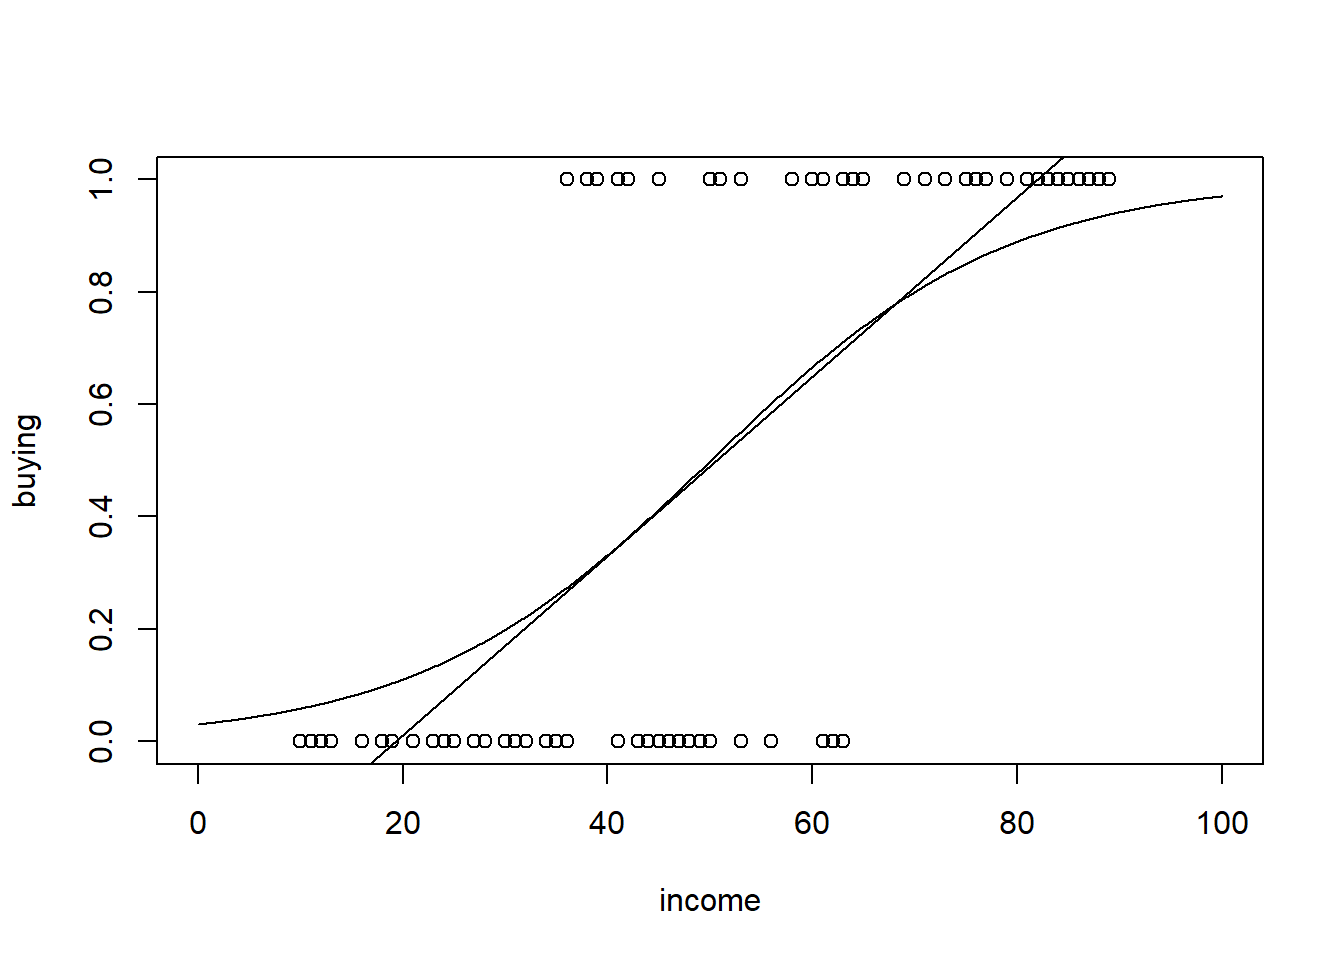
\includegraphics{bookdownproj_files/figure-latex/bcm_comparison-1.pdf}

Remember that the probability has be bounded between 0 and 1. Hence, we need to find a function \(G(z)\) such that \(0 \leq G(z) \leq 1\) for all values of \(z\) and \(P(y=1|x)=G(z)\). Popular choices for \(G(z)\) are the cumulative normal distribution function (``Probit Model'') and the logistic function (``Logit Model''). For what follows, let \(z=\beta_0+\beta_1 \cdot x_1 + \cdots + \beta_k \cdot x_k\). For the probit model, \(G(z)\) is written as
\[Pr(y = 1) = G(z)=\Phi(z)\]
where \(\Phi\) represents the cumulative normal. And for the logit model, \(G(z)\) is written as
\[Pr(y = 1) = G(z)=\frac{e^z}{1+e^z}=\frac{1}{1+e^{-z}}\]
The interpretation of the logit and probit estimates is not as straightforward as in the multivariate regression case. In general, we care about the effect of \(x\) on \(P(y=1|x)\). The sign of the coefficient shows the direction of the change in probability. The approximation to the marginal effect if \(x\) is roughly continuous:
\[\Delta P(y=1|x) \approx g(\hat{\beta}_0 + x \cdot \hat{\beta}) \cdot \beta_j \cdot \Delta x_j\]
To obtain the marginal effects in R, an additional step is necessary. Let us illustrate the binary choice model using the data set \texttt{organic} and a logit model. The results of interest for the binary choice model are the (1) coefficient estimates, (2) marginal effects, and (3) predicted probabilities.

\hypertarget{binary-choice-estimation-in-r}{%
\subsection{Binary Choice Estimation in R}\label{binary-choice-estimation-in-r}}

There are (at least) two possibilities to obtain the coefficient estimates in R. The first is using the built in R command \texttt{glm()}:

\begin{Shaded}
\begin{Highlighting}[]
\NormalTok{bhat_glm_logit =}\StringTok{ }\KeywordTok{glm}\NormalTok{(buying}\OperatorTok{~}\NormalTok{income,}\DataTypeTok{family=}\KeywordTok{binomial}\NormalTok{(}\DataTypeTok{link=}\StringTok{"logit"}\NormalTok{),}\DataTypeTok{data=}\NormalTok{organic)}
\KeywordTok{summary}\NormalTok{(bhat_glm_logit)}
\end{Highlighting}
\end{Shaded}

\begin{verbatim}
## 
## Call:
## glm(formula = buying ~ income, family = binomial(link = "logit"), 
##     data = organic)
## 
## Deviance Residuals: 
##     Min       1Q   Median       3Q      Max  
## -1.8451  -0.5293  -0.1423   0.4093   1.9154  
## 
## Coefficients:
##             Estimate Std. Error z value Pr(>|z|)    
## (Intercept) -5.87557    1.13842  -5.161 2.45e-07 ***
## income       0.11709    0.02247   5.211 1.87e-07 ***
## ---
## Signif. codes:  0 '***' 0.001 '**' 0.01 '*' 0.05 '.' 0.1 ' ' 1
## 
## (Dispersion parameter for binomial family taken to be 1)
## 
##     Null deviance: 138.469  on 99  degrees of freedom
## Residual deviance:  70.931  on 98  degrees of freedom
## AIC: 74.931
## 
## Number of Fisher Scoring iterations: 6
\end{verbatim}

Note that interpretation of the coefficients is slightly different from the regular linear model. The sign of the coefficient estimate for income is interpreted as the direction in which the probability changes. In this case, the coefficient is positive and thus, an increase (decrease) in income leads to an increase (decrease) in the probability of purchasing organic food. In addition, the coefficients are statistically significant. As aforementioned, the coefficients do not indicate the marginal effects though. To calculate the marginal effects, a slightly different approach is necessary. Let us first look at the second approach of obtaining the coefficient estimates and the R package \href{https://cran.r-project.org/web/packages/mfx/index.html}{mfx} is required to do so.

\begin{Shaded}
\begin{Highlighting}[]
\NormalTok{bhat =}\StringTok{ }\KeywordTok{logitmfx}\NormalTok{(buying}\OperatorTok{~}\NormalTok{income,}\DataTypeTok{data=}\NormalTok{organic)}
\KeywordTok{summary}\NormalTok{(bhat}\OperatorTok{$}\NormalTok{fit)}
\end{Highlighting}
\end{Shaded}

\begin{verbatim}
## 
## Call:
## glm(formula = formula, family = binomial(link = "logit"), data = data, 
##     start = start, control = control, x = T)
## 
## Deviance Residuals: 
##     Min       1Q   Median       3Q      Max  
## -1.8451  -0.5293  -0.1423   0.4093   1.9154  
## 
## Coefficients:
##             Estimate Std. Error z value Pr(>|z|)    
## (Intercept) -5.87557    1.13842  -5.161 2.45e-07 ***
## income       0.11709    0.02247   5.211 1.87e-07 ***
## ---
## Signif. codes:  0 '***' 0.001 '**' 0.01 '*' 0.05 '.' 0.1 ' ' 1
## 
## (Dispersion parameter for binomial family taken to be 1)
## 
##     Null deviance: 138.469  on 99  degrees of freedom
## Residual deviance:  70.931  on 98  degrees of freedom
## AIC: 74.931
## 
## Number of Fisher Scoring iterations: 6
\end{verbatim}

The results are identical as before using the \texttt{glm()} but the command \texttt{logitmfx()} allows for the calculation of the marginal effects as well. This is done with the command the \texttt{bhat\textbackslash{}\$mfxest}.

\begin{Shaded}
\begin{Highlighting}[]
\NormalTok{bhat}\OperatorTok{$}\NormalTok{mfxest}
\end{Highlighting}
\end{Shaded}

\begin{verbatim}
##             dF/dx   Std. Err.        z        P>|z|
## income 0.02919553 0.005634262 5.181785 2.197728e-07
\end{verbatim}

It is important to note that the marginal effects are taken at the mean of the independent variables. To calculate the marginal effects at specific points, the command \texttt{margins()} must be used. Before, we used the command \texttt{glm()} to calculate the logit coefficients. The reason for using the \texttt{glm()} is that it allows us to calculate the predicted probabilities. Consider the example to purchase organic food and assume that there are three new respondents with income levels \$25,000, \$50,000, and \$75,000. To predict the probability of those individuals purchasing organic food, the following functions can be used:

\begin{Shaded}
\begin{Highlighting}[]
\NormalTok{datablock =}\StringTok{ }\KeywordTok{data.frame}\NormalTok{(}\DataTypeTok{income=}\KeywordTok{c}\NormalTok{(}\DecValTok{25}\NormalTok{,}\DecValTok{50}\NormalTok{,}\DecValTok{75}\NormalTok{))}
\KeywordTok{predict}\NormalTok{(bhat_glm_logit,}\DataTypeTok{newdata=}\NormalTok{datablock,}\DataTypeTok{type=}\StringTok{"response"}\NormalTok{)}
\end{Highlighting}
\end{Shaded}

\begin{verbatim}
##         1         2         3 
## 0.0498116 0.4946870 0.9481377
\end{verbatim}

\hypertarget{additional-examples-and-probit-model}{%
\subsection{Additional Examples and Probit Model}\label{additional-examples-and-probit-model}}

Here are two additional examples on working full-time and voting behavior. Both examples use the \texttt{gss2018} data. Note that the previous chapter have introduced the logit model. To estimate a Probit model, the term ``logit'' has to be replaced with ``probit.'' The results are almost identical. The variables are defined as follows:

\begin{itemize}
\tightlist
\item
  \(fulltime\): Does the respondent work full time.
\item
  \(government\): Does the respondent work for the government
\item
  \(education\): Less than high school (0), high school (1), associate/junior college (2), bachelor (3), and graduate (4)
\item
  \(vote\): Voted in the 2016 election
\item
  \(married\), \(age\), \(childs\), and \(income\) are self-explanatory. Income is for 2016.
\end{itemize}

\hypertarget{full-time-work}{%
\subsubsection{Full-Time Work}\label{full-time-work}}

\begin{Shaded}
\begin{Highlighting}[]
\NormalTok{equation =}\StringTok{ }\KeywordTok{c}\NormalTok{(}\StringTok{"fulltime~age+childs+government+education+married"}\NormalTok{)}
\NormalTok{bhat_glm =}\StringTok{ }\KeywordTok{glm}\NormalTok{(equation,}\DataTypeTok{family=}\KeywordTok{binomial}\NormalTok{(}\DataTypeTok{link=}\StringTok{"logit"}\NormalTok{),}\DataTypeTok{data=}\NormalTok{gss2018)}
\KeywordTok{summary}\NormalTok{(bhat_glm)}
\end{Highlighting}
\end{Shaded}

\begin{verbatim}
## 
## Call:
## glm(formula = equation, family = binomial(link = "logit"), data = gss2018)
## 
## Deviance Residuals: 
##     Min       1Q   Median       3Q      Max  
## -2.3019   0.4298   0.5638   0.6692   0.9954  
## 
## Coefficients:
##              Estimate Std. Error z value Pr(>|z|)    
## (Intercept)  1.877519   0.335655   5.594 2.22e-08 ***
## age         -0.021941   0.006985  -3.141  0.00168 ** 
## childs      -0.015773   0.063675  -0.248  0.80435    
## government   0.323365   0.272825   1.185  0.23592    
## education    0.264400   0.086471   3.058  0.00223 ** 
## married      0.353223   0.205331   1.720  0.08539 .  
## ---
## Signif. codes:  0 '***' 0.001 '**' 0.01 '*' 0.05 '.' 0.1 ' ' 1
## 
## (Dispersion parameter for binomial family taken to be 1)
## 
##     Null deviance: 724.91  on 771  degrees of freedom
## Residual deviance: 699.31  on 766  degrees of freedom
## AIC: 711.31
## 
## Number of Fisher Scoring iterations: 4
\end{verbatim}

\begin{Shaded}
\begin{Highlighting}[]
\NormalTok{bhat =}\StringTok{ }\KeywordTok{logitmfx}\NormalTok{(equation,}\DataTypeTok{data=}\NormalTok{gss2018)}
\KeywordTok{summary}\NormalTok{(bhat}\OperatorTok{$}\NormalTok{fit)}
\end{Highlighting}
\end{Shaded}

\begin{verbatim}
## 
## Call:
## glm(formula = formula, family = binomial(link = "logit"), data = data, 
##     start = start, control = control, x = T)
## 
## Deviance Residuals: 
##     Min       1Q   Median       3Q      Max  
## -2.3019   0.4298   0.5638   0.6692   0.9954  
## 
## Coefficients:
##              Estimate Std. Error z value Pr(>|z|)    
## (Intercept)  1.877519   0.335655   5.594 2.22e-08 ***
## age         -0.021941   0.006985  -3.141  0.00168 ** 
## childs      -0.015773   0.063675  -0.248  0.80435    
## government   0.323365   0.272825   1.185  0.23592    
## education    0.264400   0.086471   3.058  0.00223 ** 
## married      0.353223   0.205331   1.720  0.08539 .  
## ---
## Signif. codes:  0 '***' 0.001 '**' 0.01 '*' 0.05 '.' 0.1 ' ' 1
## 
## (Dispersion parameter for binomial family taken to be 1)
## 
##     Null deviance: 724.91  on 771  degrees of freedom
## Residual deviance: 699.31  on 766  degrees of freedom
## AIC: 711.31
## 
## Number of Fisher Scoring iterations: 4
\end{verbatim}

\begin{Shaded}
\begin{Highlighting}[]
\NormalTok{bhat_glm =}\StringTok{ }\KeywordTok{glm}\NormalTok{(equation,}\DataTypeTok{family=}\KeywordTok{binomial}\NormalTok{(}\DataTypeTok{link=}\StringTok{"probit"}\NormalTok{),}\DataTypeTok{data=}\NormalTok{gss2018)}
\KeywordTok{summary}\NormalTok{(bhat_glm)}
\end{Highlighting}
\end{Shaded}

\begin{verbatim}
## 
## Call:
## glm(formula = equation, family = binomial(link = "probit"), data = gss2018)
## 
## Deviance Residuals: 
##     Min       1Q   Median       3Q      Max  
## -2.3240   0.4189   0.5671   0.6720   0.9792  
## 
## Coefficients:
##              Estimate Std. Error z value Pr(>|z|)    
## (Intercept)  1.087820   0.187423   5.804 6.47e-09 ***
## age         -0.011979   0.003992  -3.001  0.00269 ** 
## childs      -0.008966   0.036310  -0.247  0.80496    
## government   0.172189   0.148316   1.161  0.24566    
## education    0.154238   0.047653   3.237  0.00121 ** 
## married      0.196650   0.114850   1.712  0.08686 .  
## ---
## Signif. codes:  0 '***' 0.001 '**' 0.01 '*' 0.05 '.' 0.1 ' ' 1
## 
## (Dispersion parameter for binomial family taken to be 1)
## 
##     Null deviance: 724.91  on 771  degrees of freedom
## Residual deviance: 699.29  on 766  degrees of freedom
## AIC: 711.29
## 
## Number of Fisher Scoring iterations: 5
\end{verbatim}

\hypertarget{voting-behavior}{%
\subsubsection{Voting Behavior}\label{voting-behavior}}

\begin{Shaded}
\begin{Highlighting}[]
\NormalTok{equation =}\StringTok{ }\KeywordTok{c}\NormalTok{(}\StringTok{"vote~age+childs+government+education+married+income"}\NormalTok{)}
\NormalTok{bhat_glm =}\StringTok{ }\KeywordTok{glm}\NormalTok{(equation,}\DataTypeTok{family=}\KeywordTok{binomial}\NormalTok{(}\DataTypeTok{link=}\StringTok{"logit"}\NormalTok{),}\DataTypeTok{data=}\NormalTok{gss2018)}
\KeywordTok{summary}\NormalTok{(bhat_glm)}
\end{Highlighting}
\end{Shaded}

\begin{verbatim}
## 
## Call:
## glm(formula = equation, family = binomial(link = "logit"), data = gss2018)
## 
## Deviance Residuals: 
##     Min       1Q   Median       3Q      Max  
## -2.3291  -1.0702   0.5551   0.8683   1.6618  
## 
## Coefficients:
##               Estimate Std. Error z value Pr(>|z|)    
## (Intercept) -1.924e+00  2.983e-01  -6.449 1.13e-10 ***
## age          4.145e-02  6.944e-03   5.970 2.37e-09 ***
## childs      -7.944e-02  5.677e-02  -1.399    0.162    
## government   4.536e-01  2.325e-01   1.951    0.051 .  
## education    4.923e-01  8.326e-02   5.913 3.36e-09 ***
## married      1.282e-01  1.779e-01   0.721    0.471    
## income       2.039e-06  2.470e-06   0.826    0.409    
## ---
## Signif. codes:  0 '***' 0.001 '**' 0.01 '*' 0.05 '.' 0.1 ' ' 1
## 
## (Dispersion parameter for binomial family taken to be 1)
## 
##     Null deviance: 978.09  on 771  degrees of freedom
## Residual deviance: 858.90  on 765  degrees of freedom
## AIC: 872.9
## 
## Number of Fisher Scoring iterations: 4
\end{verbatim}

\begin{Shaded}
\begin{Highlighting}[]
\NormalTok{bhat =}\StringTok{ }\KeywordTok{logitmfx}\NormalTok{(equation,}\DataTypeTok{data=}\NormalTok{gss2018)}
\KeywordTok{summary}\NormalTok{(bhat}\OperatorTok{$}\NormalTok{fit)}
\end{Highlighting}
\end{Shaded}

\begin{verbatim}
## 
## Call:
## glm(formula = formula, family = binomial(link = "logit"), data = data, 
##     start = start, control = control, x = T)
## 
## Deviance Residuals: 
##     Min       1Q   Median       3Q      Max  
## -2.3291  -1.0702   0.5551   0.8683   1.6618  
## 
## Coefficients:
##               Estimate Std. Error z value Pr(>|z|)    
## (Intercept) -1.924e+00  2.983e-01  -6.449 1.13e-10 ***
## age          4.145e-02  6.944e-03   5.970 2.37e-09 ***
## childs      -7.944e-02  5.677e-02  -1.399    0.162    
## government   4.536e-01  2.325e-01   1.951    0.051 .  
## education    4.923e-01  8.326e-02   5.913 3.36e-09 ***
## married      1.282e-01  1.779e-01   0.721    0.471    
## income       2.039e-06  2.470e-06   0.826    0.409    
## ---
## Signif. codes:  0 '***' 0.001 '**' 0.01 '*' 0.05 '.' 0.1 ' ' 1
## 
## (Dispersion parameter for binomial family taken to be 1)
## 
##     Null deviance: 978.09  on 771  degrees of freedom
## Residual deviance: 858.90  on 765  degrees of freedom
## AIC: 872.9
## 
## Number of Fisher Scoring iterations: 4
\end{verbatim}

\begin{Shaded}
\begin{Highlighting}[]
\NormalTok{bhat_glm =}\StringTok{ }\KeywordTok{glm}\NormalTok{(equation,}\DataTypeTok{family=}\KeywordTok{binomial}\NormalTok{(}\DataTypeTok{link=}\StringTok{"probit"}\NormalTok{),}\DataTypeTok{data=}\NormalTok{gss2018)}
\KeywordTok{summary}\NormalTok{(bhat_glm)}
\end{Highlighting}
\end{Shaded}

\begin{verbatim}
## 
## Call:
## glm(formula = equation, family = binomial(link = "probit"), data = gss2018)
## 
## Deviance Residuals: 
##     Min       1Q   Median       3Q      Max  
## -2.3910  -1.0777   0.5492   0.8754   1.6541  
## 
## Coefficients:
##               Estimate Std. Error z value Pr(>|z|)    
## (Intercept) -1.167e+00  1.771e-01  -6.589 4.43e-11 ***
## age          2.527e-02  4.055e-03   6.232 4.60e-10 ***
## childs      -4.884e-02  3.411e-02  -1.432   0.1522    
## government   2.722e-01  1.359e-01   2.003   0.0452 *  
## education    2.949e-01  4.830e-02   6.106 1.02e-09 ***
## married      8.745e-02  1.062e-01   0.824   0.4101    
## income       1.132e-06  1.435e-06   0.789   0.4302    
## ---
## Signif. codes:  0 '***' 0.001 '**' 0.01 '*' 0.05 '.' 0.1 ' ' 1
## 
## (Dispersion parameter for binomial family taken to be 1)
## 
##     Null deviance: 978.09  on 771  degrees of freedom
## Residual deviance: 857.62  on 765  degrees of freedom
## AIC: 871.62
## 
## Number of Fisher Scoring iterations: 4
\end{verbatim}

\hypertarget{exercises-2}{%
\subsection{Exercises}\label{exercises-2}}

\begin{enumerate}
\def\labelenumi{\arabic{enumi}.}
\item
  Consider the problem of choosing whether or not to purchase a hybrid vehicle (e.g., the Toyota Prius, Honda Civic Hybrid, Ford Escape). As an analyst, you assume that whether or not an individual purchases a hybrid depends upon the current price of gasoline (\emph{gas}), the difference in purchase price of a hybrid vehicle compared to a comparably equipped vehicle (\emph{increment}), college education which is represented by a dummy variable that equals 1 if individual has completed college and equals 0 otherwise (\(college\)), and a dummy variable that equals 1 if the individual is a member of an environmental organization, e.g., Nature Conservancy, National Audubon Society, (\emph{env}). Answer the following questions contained in \texttt{hybrid}:

  \begin{enumerate}
  \def\labelenumii{\alph{enumii}.}
  \item
    Provide summary statistics (i.e., mean, minimum, and maximum) for each variables.
  \item
    Estimate a regression model that allows to calculate the probability that a person would buy a hybrid.
  \item
    Using your parameter estimates, compute the probability that the following ``types'' of individuals will buy a hybrid:

    \begin{itemize}
    \tightlist
    \item
      Type I: gasoline price = 2.50; difference in purchase price = 1,500; college = 0; and member of an environmental organization = 0
    \item
      Type II: gasoline price = 3.50; difference in purchase price = 500; college = 1; and member of an environmental organization = 1
    \item
      Type III: gasoline price = 3.00; difference in purchase price = 1,000; college = 1; and member of an environmental organization = 0
    \end{itemize}
  \item
    Given the above probabilities, calculate the marginal effect that gasoline prices have on the probability that each of the three ``types'' of individuals will purchase a hybrid vehicle.
  \item
    Given the above probabilities, calculate the marginal effect that joining an environmental group on Type I and Type III individuals.
  \end{enumerate}
\item
  \emph{EV Data}: Using the \texttt{evdata}, estimate a logit model which calculates the probability that a consumer would purchase a hybrid (choice=2), plug-in hybrid (choice=3), or electric vehicle (choice=4) as opposed to a gasoline car (choice=1). In a first step, you should create a new variable that is equal to 0 if the person purchases a gasoline vehicle and is equal to 1 for everything else. Include the following independent variables in your model: \(age\), \(numcars\), \(politics\), \(female\), \(edu\), and \(income\).
\item
  We are interested in the determinants of voting based on data from the General Social Survey (GSS). The following variables are hypothesized to be a determinant of voting behavior: \(age\), \(income\), \(gun ownership\) (yes=1), \(stance on death penalty\) (in favor=1), and \(education level\) (higher number is associated with a higher education level). Run a probit and logit model and report the results. Calculate the marginal probabilities.
\end{enumerate}

\textbackslash end\{enumerate\}

\hypertarget{qualitative-choice-models}{%
\section{Qualitative Choice Models}\label{qualitative-choice-models}}

The packages required for this section are \texttt{mlogit}, \texttt{erer}, \texttt{MASS}, \texttt{AER}, \texttt{glmmML}, and \texttt{nnet}. The files required are \texttt{fpdata} and \texttt{evdata}. Additional files that are required are part of the packages \href{https://cran.r-project.org/web/packages/mlogit/index.html}{mlogit} and \href{https://cran.r-project.org/web/packages/AER/index.html}{AER}. Those datasets are called \texttt{Fishing} and \texttt{TravelMode}. You can lode them into R with the following commands:

\begin{itemize}
\tightlist
\item
  \texttt{data("Fishing",package="mlogit")}
\item
  \texttt{data("TravelMode",package="AER")}
\end{itemize}

There is also a \href{https://youtu.be/xLUIil1sGW4}{YouTube Video} associated with this chapter.

The last chapter has introduced binary choice models that answer questions such as:

\begin{itemize}
\tightlist
\item
  Did you vote during the last election?
\item
  Does an individual recidivate after being released from prison?
\end{itemize}

In this chapter, cases of dependent variables with more than two categories are considered. The categorical dependent variables can be with or without natural ordering. Here are some examples of natural ordering:

\begin{itemize}
\tightlist
\item
  Level of happiness: Very happy, happy, okay, or sad
\item
  Intent to get vaccinated: Definitely yes, probably yes, probably no, definitely no
\end{itemize}

Examples without natural ordering:

\begin{itemize}
\tightlist
\item
  Type of car to purchase: Passenger car, Pick-up truck, van, convertible
\end{itemize}

\hypertarget{ordered-logit-model}{%
\subsection{Ordered Logit Model}\label{ordered-logit-model}}

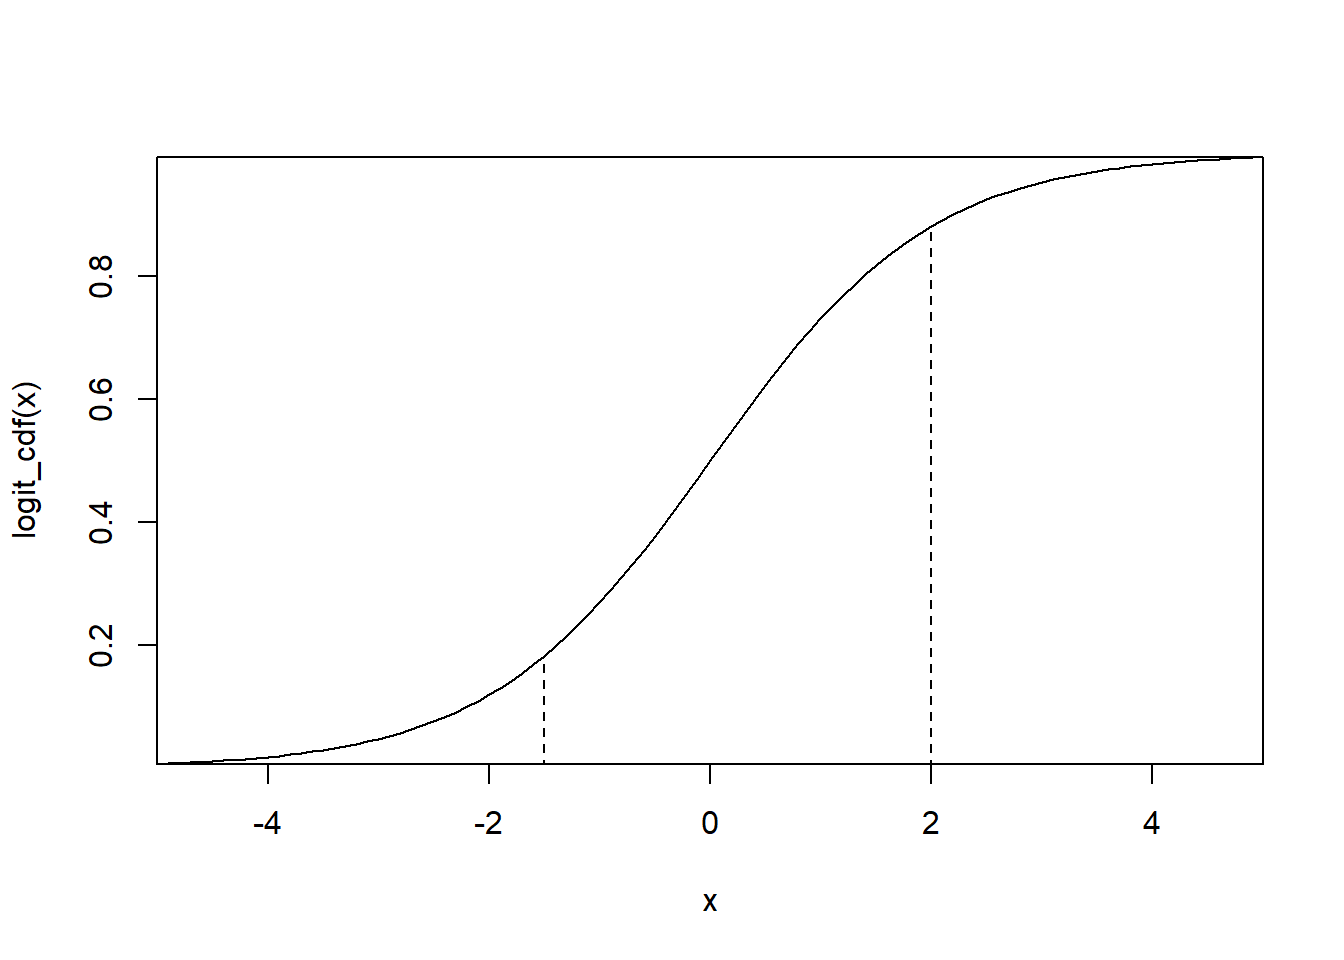
\includegraphics{bookdownproj_files/figure-latex/ordered_logit_plot-1.pdf}

\hypertarget{theoretical-aspects}{%
\subsubsection{Theoretical Aspects}\label{theoretical-aspects}}

Assumption: Latent variable \(y^*\) that is unobserved by the researcher:
\[y_i^* = \beta_0+\beta_1 \cdot x_i + \epsilon_i\]
In the case of a health model, this may be a measure of healthiness. What the researcher does measure is an \(m\)-alternative ordered model:
\[y_i = j \quad \text{if} \quad \alpha_{j-1} < y_i^* \leq \alpha_j \quad \text{for} \quad  j=1, \dots,m\]
where \(\alpha_0 = - \infty\) and \(\alpha_m=\infty\). In this case, we have
\[ \begin{align*}
    Pr(y_1 = j) &=Pr(\alpha_{j-1} < y_i^* \leq \alpha_j)\\
                &=Pr(\alpha_{j-1} < \beta_0+\beta_1 x_i + \epsilon_i \leq \alpha_j)\\
                &=Pr(\alpha_{j-1}- \beta_0-\beta_1 x_i < \epsilon_i \leq \alpha_j - \beta_0-\beta_1 x_i)\\
                        &=F(\alpha_j - \beta_0-\beta_1 x_i)-F(\alpha_{j-1} - \beta_0-\beta_1 x_i)
    \end{align*}\]
For the ordered logit: \(F(z)=exp(z)/(1+exp(z))\). Cut-off example points as \(\alpha_0 = -\infty\), \(\alpha_2 = -1.5\), \(\alpha_3 = 2\), and \(\alpha_4 = \infty\)

\hypertarget{ordered-logit-example-organic-food-purchase}{%
\subsubsection{Ordered Logit Example: Organic Food Purchase}\label{ordered-logit-example-organic-food-purchase}}

Survey on the purchase frequency of organic tomatoes and organic strawberries \texttt{fpdata.csv}:

\begin{itemize}
\tightlist
\item
  Never (1), rarely (2), once per month (3), every 2 weeks (4), 1-2 times a week (5), almost daily (6)
\end{itemize}

Independent variables are

-Age and female
- Education: High school (1), some college (2), bachelor (3), master (4), technical school diploma (5), doctorate (6)

\begin{Shaded}
\begin{Highlighting}[]
\NormalTok{fpdata}\OperatorTok{$}\NormalTok{strawberries_org =}\StringTok{ }\KeywordTok{as.factor}\NormalTok{(fpdata}\OperatorTok{$}\NormalTok{strawberries_org)}
\NormalTok{strawdata  =}\StringTok{ }\NormalTok{fpdata[}\KeywordTok{c}\NormalTok{(}\StringTok{"strawberries_org"}\NormalTok{,}\StringTok{"age"}\NormalTok{,}\StringTok{"education"}\NormalTok{,}\StringTok{"female"}\NormalTok{,}\StringTok{"kidsunder12"}\NormalTok{)]}
\NormalTok{strawdata  =}\StringTok{ }\KeywordTok{na.omit}\NormalTok{(strawdata)}
\NormalTok{bhat =}\StringTok{ }\KeywordTok{polr}\NormalTok{(strawberries_org}\OperatorTok{~}\NormalTok{age}\OperatorTok{+}\NormalTok{education}\OperatorTok{+}\NormalTok{female}\OperatorTok{+}\NormalTok{kidsunder12,}\DataTypeTok{data=}\NormalTok{strawdata,}\DataTypeTok{Hess=}\OtherTok{TRUE}\NormalTok{)}
\KeywordTok{summary}\NormalTok{(bhat)}
\end{Highlighting}
\end{Shaded}

\begin{verbatim}
## Call:
## polr(formula = strawberries_org ~ age + education + female + 
##     kidsunder12, data = strawdata, Hess = TRUE)
## 
## Coefficients:
##                Value Std. Error t value
## age         -0.02034   0.009838 -2.0676
## education    0.01596   0.112028  0.1425
## female      -0.41533   0.280485 -1.4808
## kidsunder12  0.28560   0.321778  0.8876
## 
## Intercepts:
##     Value   Std. Error t value
## 0|1 -1.4958  0.6497    -2.3022
## 1|2 -0.4381  0.6434    -0.6810
## 2|3  0.2084  0.6394     0.3259
## 3|4  0.8352  0.6442     1.2964
## 4|5  1.6314  0.6699     2.4353
## 
## Residual Deviance: 526.4547 
## AIC: 544.4547
\end{verbatim}

For the organic purchases data, the cuts are under ``Intercepts'' and thus, we have (rounded coefficients):
\[z =  -0.020 \cdot age  +0.0160 \cdot education -0.415 \cdot female +0.286 \cdot kidsunder12\]
The cutoff points can be interpreted as follows:
\[\begin{align*}
    Pr(y=1) &= P(z+\epsilon_i \leq -1.4958)\\
    Pr(y=2) &= P(-1.4958 < z+\epsilon_i \leq -0.4381)\\
    Pr(y=3) &= P(-0.4381 < z+\epsilon_i \leq  0.2084)\\
    Pr(y=4) &= P(0.2084 < z+\epsilon_i \leq 0.8352)\\
    Pr(y=4) &= P(0.8352 < z+\epsilon_i \leq 1.6314)\\
    Pr(y=6) &= P(1.6314 \leq z+\epsilon_i )
\end{align*}\]
In order to get the \(p\)-values displayed in the output, you have to execute two additional steps:

\begin{Shaded}
\begin{Highlighting}[]
\NormalTok{bhat.coef =}\StringTok{ }\KeywordTok{data.frame}\NormalTok{(}\KeywordTok{coef}\NormalTok{(}\KeywordTok{summary}\NormalTok{(bhat)))}
\NormalTok{bhat.coef}\OperatorTok{$}\NormalTok{pval =}\StringTok{ }\KeywordTok{round}\NormalTok{((}\KeywordTok{pnorm}\NormalTok{(}\KeywordTok{abs}\NormalTok{(bhat.coef}\OperatorTok{$}\NormalTok{t.value), }\DataTypeTok{lower.tail =} \OtherTok{FALSE}\NormalTok{) }\OperatorTok{*}\StringTok{ }\DecValTok{2}\NormalTok{),}\DecValTok{2}\NormalTok{)}
\NormalTok{bhat.coef}
\end{Highlighting}
\end{Shaded}

\begin{verbatim}
##                   Value  Std..Error    t.value pval
## age         -0.02034185 0.009838336 -2.0676110 0.04
## education    0.01595914 0.112027882  0.1424569 0.89
## female      -0.41533145 0.280485372 -1.4807598 0.14
## kidsunder12  0.28560319 0.321777883  0.8875787 0.37
## 0|1         -1.49575271 0.649708891 -2.3021891 0.02
## 1|2         -0.43813109 0.643390358 -0.6809724 0.50
## 2|3          0.20839939 0.639383205  0.3259382 0.74
## 3|4          0.83515493 0.644195302  1.2964313 0.19
## 4|5          1.63135404 0.669870994  2.4353257 0.01
\end{verbatim}

\hypertarget{predicted-probability-and-marginal-effects}{%
\subsubsection{Predicted Probability and Marginal Effects}\label{predicted-probability-and-marginal-effects}}

The predicted probability for each observation can be obtained using the command \texttt{predict(bhat,type="probs")} assuming that the output of the \texttt{polr} command is stored in \emph{bhat}.

\begin{Shaded}
\begin{Highlighting}[]
\NormalTok{bhat.pred =}\StringTok{ }\KeywordTok{predict}\NormalTok{(bhat, }\DataTypeTok{type=}\StringTok{"probs"}\NormalTok{)}
\NormalTok{x =}\StringTok{ }\KeywordTok{ocME}\NormalTok{(bhat)}
\NormalTok{x}\OperatorTok{$}\NormalTok{out}\OperatorTok{$}\NormalTok{ME.all}
\end{Highlighting}
\end{Shaded}

\begin{verbatim}
##             effect.0 effect.1 effect.2 effect.3 effect.4 effect.5
## age            0.005    0.000   -0.001   -0.001   -0.001   -0.001
## education     -0.004    0.000    0.001    0.001    0.001    0.001
## female         0.098   -0.003   -0.023   -0.024   -0.023   -0.026
## kidsunder12   -0.067    0.001    0.015    0.017    0.016    0.018
\end{verbatim}

\hypertarget{multinomial-logit-and-multinomial-probit-models}{%
\subsection{Multinomial Logit and Multinomial Probit Models}\label{multinomial-logit-and-multinomial-probit-models}}

Revealed preferences:

\begin{itemize}
\tightlist
\item
  Observed choices of individuals
\end{itemize}

Stated preference

\begin{itemize}
\tightlist
\item
  Hypothetical choice situations
\end{itemize}

Economists' modeling of choice

\begin{itemize}
\tightlist
\item
  Utility/happiness/satisfaction associated with multiple choice situations
\end{itemize}

\hypertarget{theoretical-aspects-1}{%
\subsubsection{Theoretical Aspects}\label{theoretical-aspects-1}}

Travel choice model dependent on cost (\(x\)) and time (\(z\)):
\[V_j = \alpha_j + \beta_1 \cdot x_j + \beta_2 \cdot z_j\]
Probability of choosing alternative \(j\) (assuming three choices)
\[\begin{align*}
    P(1) &= \frac{e^{V_1}}{e^{V_1}+e^{V_2}+e^{V_3}}\\
    P(2) &= \frac{e^{V_2}}{e^{V_1}+e^{V_2}+e^{V_3}}\\
    P(3) &= \frac{e^{V_3}}{e^{V_1}+e^{V_2}+e^{V_3}}
\end{align*}\]
Note that \(P(1)+P(2)+P(3) = 1\)

\hypertarget{data-managment}{%
\subsubsection{Data Managment}\label{data-managment}}

Long shape

\begin{itemize}
\tightlist
\item
  One row for each alternative
\end{itemize}

Wide shape

\begin{itemize}
\tightlist
\item
  One row for each choice situation
\end{itemize}

There are some very good resources on data management and the package in general:

\begin{itemize}
\tightlist
\item
  \href{http://dx.doi.org/10.18637/jss.v095.i11}{Estimation of Random Utility Models in R: The mlogit Package}
\end{itemize}

Fishing (wide format)

\begin{itemize}
\tightlist
\item
  Fishing modes: beach, pier, private, and charter
\item
  Alternative-specific variables: price and catch
\item
  Individual-specific variables: income
\item
  Suitability of the ``wide'' format to store individual-specific variables
\item
  The R parameter \texttt{varying} designates alternative specific variables
\end{itemize}

Travel Mode (long format)

\begin{itemize}
\tightlist
\item
  \href{https://rdrr.io/cran/AER/man/TravelMode.html}{Travel Mode Choice Data}
\item
  \texttt{mlogit.data(travelmode,choice="choice",shape="long",\ alt.levels=c("air","train","bus","car"))}
\end{itemize}

\hypertarget{fishing-data}{%
\subsubsection{Fishing Data}\label{fishing-data}}

\begin{Shaded}
\begin{Highlighting}[]
\KeywordTok{data}\NormalTok{(}\StringTok{"Fishing"}\NormalTok{,}\DataTypeTok{package=}\StringTok{"mlogit"}\NormalTok{)}
\NormalTok{fishing             =}\StringTok{ }\KeywordTok{mlogit.data}\NormalTok{(Fishing,}\DataTypeTok{shape=}\StringTok{"wide"}\NormalTok{,}\DataTypeTok{varying=}\DecValTok{2}\OperatorTok{:}\DecValTok{9}\NormalTok{,}\DataTypeTok{choice=}\StringTok{"mode"}\NormalTok{)}
\NormalTok{bhat                =}\StringTok{ }\KeywordTok{mlogit}\NormalTok{(mode}\OperatorTok{~}\DecValTok{0}\OperatorTok{|}\NormalTok{income,fishing)}
\KeywordTok{summary}\NormalTok{(bhat)}
\end{Highlighting}
\end{Shaded}

\begin{verbatim}
## 
## Call:
## mlogit(formula = mode ~ 0 | income, data = fishing, method = "nr")
## 
## Frequencies of alternatives:choice
##   beach    boat charter    pier 
## 0.11337 0.35364 0.38240 0.15059 
## 
## nr method
## 4 iterations, 0h:0m:0s 
## g'(-H)^-1g = 8.32E-07 
## gradient close to zero 
## 
## Coefficients :
##                        Estimate  Std. Error z-value  Pr(>|z|)    
## (Intercept):boat     7.3892e-01  1.9673e-01  3.7560 0.0001727 ***
## (Intercept):charter  1.3413e+00  1.9452e-01  6.8955 5.367e-12 ***
## (Intercept):pier     8.1415e-01  2.2863e-01  3.5610 0.0003695 ***
## income:boat          9.1906e-05  4.0664e-05  2.2602 0.0238116 *  
## income:charter      -3.1640e-05  4.1846e-05 -0.7561 0.4495908    
## income:pier         -1.4340e-04  5.3288e-05 -2.6911 0.0071223 ** 
## ---
## Signif. codes:  0 '***' 0.001 '**' 0.01 '*' 0.05 '.' 0.1 ' ' 1
## 
## Log-Likelihood: -1477.2
## McFadden R^2:  0.013736 
## Likelihood ratio test : chisq = 41.145 (p.value = 6.0931e-09)
\end{verbatim}

\begin{Shaded}
\begin{Highlighting}[]
\NormalTok{fishing.fitted      =}\StringTok{ }\KeywordTok{fitted}\NormalTok{(bhat,}\DataTypeTok{outcome=}\OtherTok{FALSE}\NormalTok{)}
\KeywordTok{effects}\NormalTok{(bhat,}\DataTypeTok{covariate =}\StringTok{"income"}\NormalTok{)}
\end{Highlighting}
\end{Shaded}

\begin{verbatim}
##         beach          boat       charter          pier 
##  7.496226e-08  3.259851e-05 -1.201366e-05 -2.065981e-05
\end{verbatim}

\begin{Shaded}
\begin{Highlighting}[]
\NormalTok{bhat                =}\StringTok{ }\KeywordTok{mlogit}\NormalTok{(mode}\OperatorTok{~}\NormalTok{catch}\OperatorTok{+}\NormalTok{price}\OperatorTok{|}\NormalTok{income,}\DataTypeTok{data=}\NormalTok{fishing)}
\KeywordTok{summary}\NormalTok{(bhat)}
\end{Highlighting}
\end{Shaded}

\begin{verbatim}
## 
## Call:
## mlogit(formula = mode ~ catch + price | income, data = fishing, 
##     method = "nr")
## 
## Frequencies of alternatives:choice
##   beach    boat charter    pier 
## 0.11337 0.35364 0.38240 0.15059 
## 
## nr method
## 7 iterations, 0h:0m:0s 
## g'(-H)^-1g = 1.37E-05 
## successive function values within tolerance limits 
## 
## Coefficients :
##                        Estimate  Std. Error  z-value  Pr(>|z|)    
## (Intercept):boat     5.2728e-01  2.2279e-01   2.3667 0.0179485 *  
## (Intercept):charter  1.6944e+00  2.2405e-01   7.5624 3.952e-14 ***
## (Intercept):pier     7.7796e-01  2.2049e-01   3.5283 0.0004183 ***
## catch                3.5778e-01  1.0977e-01   3.2593 0.0011170 ** 
## price               -2.5117e-02  1.7317e-03 -14.5042 < 2.2e-16 ***
## income:boat          8.9440e-05  5.0067e-05   1.7864 0.0740345 .  
## income:charter      -3.3292e-05  5.0341e-05  -0.6613 0.5084031    
## income:pier         -1.2758e-04  5.0640e-05  -2.5193 0.0117582 *  
## ---
## Signif. codes:  0 '***' 0.001 '**' 0.01 '*' 0.05 '.' 0.1 ' ' 1
## 
## Log-Likelihood: -1215.1
## McFadden R^2:  0.18868 
## Likelihood ratio test : chisq = 565.17 (p.value = < 2.22e-16)
\end{verbatim}

\begin{Shaded}
\begin{Highlighting}[]
\NormalTok{fishing.fitted      =}\StringTok{ }\KeywordTok{fitted}\NormalTok{(bhat,}\DataTypeTok{outcome=}\OtherTok{FALSE}\NormalTok{)}
\KeywordTok{effects}\NormalTok{(bhat,}\DataTypeTok{covariate=}\StringTok{"income"}\NormalTok{)}
\end{Highlighting}
\end{Shaded}

\begin{verbatim}
##         beach          boat       charter          pier 
## -7.214167e-07  3.176132e-05 -2.173392e-05 -9.305980e-06
\end{verbatim}

\begin{Shaded}
\begin{Highlighting}[]
\KeywordTok{rm}\NormalTok{(bhat,Fishing,fishing,fishing.fitted)}
\end{Highlighting}
\end{Shaded}

\hypertarget{travel-data}{%
\subsubsection{Travel Data}\label{travel-data}}

\begin{Shaded}
\begin{Highlighting}[]
\KeywordTok{data}\NormalTok{(}\StringTok{"TravelMode"}\NormalTok{,}\DataTypeTok{package=}\StringTok{"AER"}\NormalTok{)}
\NormalTok{travelmode     =}\StringTok{ }\KeywordTok{mlogit.data}\NormalTok{(TravelMode,}\DataTypeTok{choice=}\StringTok{"choice"}\NormalTok{,}\DataTypeTok{shape=}\StringTok{"long"}\NormalTok{,}\DataTypeTok{alt.var=}\StringTok{"mode"}\NormalTok{)}
\NormalTok{bhat           =}\StringTok{ }\KeywordTok{mlogit}\NormalTok{(choice}\OperatorTok{~}\NormalTok{gcost}\OperatorTok{+}\NormalTok{wait}\OperatorTok{|}\NormalTok{income}\OperatorTok{+}\NormalTok{size,}\DataTypeTok{data=}\NormalTok{travelmode,}\DataTypeTok{reflevel=}\StringTok{"car"}\NormalTok{)}
\KeywordTok{summary}\NormalTok{(bhat)}
\end{Highlighting}
\end{Shaded}

\begin{verbatim}
## 
## Call:
## mlogit(formula = choice ~ gcost + wait | income + size, data = travelmode, 
##     reflevel = "car", method = "nr")
## 
## Frequencies of alternatives:choice
##     car     air   train     bus 
## 0.28095 0.27619 0.30000 0.14286 
## 
## nr method
## 5 iterations, 0h:0m:0s 
## g'(-H)^-1g = 1.66E-07 
## gradient close to zero 
## 
## Coefficients :
##                     Estimate Std. Error z-value  Pr(>|z|)    
## (Intercept):air    7.8736084  0.9868475  7.9785 1.554e-15 ***
## (Intercept):train  5.5592051  0.6991387  7.9515 1.776e-15 ***
## (Intercept):bus    4.4331916  0.7783339  5.6957 1.228e-08 ***
## gcost             -0.0196850  0.0054015 -3.6444 0.0002680 ***
## wait              -0.1015659  0.0112306 -9.0436 < 2.2e-16 ***
## income:air         0.0040710  0.0127247  0.3199 0.7490196    
## income:train      -0.0551849  0.0144824 -3.8105 0.0001387 ***
## income:bus        -0.0233237  0.0162973 -1.4311 0.1523914    
## size:air          -1.0274229  0.2656569 -3.8675 0.0001100 ***
## size:train         0.3023954  0.2256155  1.3403 0.1801437    
## size:bus          -0.0300096  0.3339774 -0.0899 0.9284023    
## ---
## Signif. codes:  0 '***' 0.001 '**' 0.01 '*' 0.05 '.' 0.1 ' ' 1
## 
## Log-Likelihood: -177.45
## McFadden R^2:  0.37463 
## Likelihood ratio test : chisq = 212.61 (p.value = < 2.22e-16)
\end{verbatim}

\begin{Shaded}
\begin{Highlighting}[]
\NormalTok{tavel.fitted =}\StringTok{ }\KeywordTok{fitted}\NormalTok{(bhat,}\DataTypeTok{outcome=}\OtherTok{FALSE}\NormalTok{)}
\end{Highlighting}
\end{Shaded}

\hypertarget{electric-vehicle-data}{%
\subsubsection{Electric Vehicle Data}\label{electric-vehicle-data}}

\begin{itemize}
\tightlist
\item
  \texttt{spendongas} (Gasoline expenditure per month in \$): 0-74 (1), 75-149 (2), 150-249 (3), 250-349 (4), 350-449 (5), 450-599 (6), and above 600 (7)
\item
  \texttt{politics} (Political position): Extremely liberal (1), liberal (2), slightly liberal (3), moderate (4), slightly conservative (5), conservative (6), and extremely conservative (7)
\item
  \texttt{Education}: Less than HS (1), HS/GED (2), some college (3), 2-year college degree (4), 4-year college degree (5), or graduate school (6)
\item
  \texttt{Income\ (1,000\ \textbackslash{}\$)}: Under 15 (1), 15 \(<\) 25 (2), 25 \(<\) 35 (3), 35 \(<\) 50 (4), 50 \(<\) 75 (5), 75 \(<\) 100 (6), 100 \(<\) 150 (7), 150 \(<\) 200 (8), 200 \(<\) 250 (9), \(>\) 250 (10)
\end{itemize}

\begin{Shaded}
\begin{Highlighting}[]
\NormalTok{evdata =}\StringTok{ }\KeywordTok{mlogit.data}\NormalTok{(evdata,}\DataTypeTok{shape=}\StringTok{"wide"}\NormalTok{,}\DataTypeTok{choice=}\StringTok{"choice"}\NormalTok{)}
\NormalTok{bhat =}\StringTok{ }\KeywordTok{mlogit}\NormalTok{(choice}\OperatorTok{~}\DecValTok{0}\OperatorTok{|}\NormalTok{age}\OperatorTok{+}\NormalTok{female}\OperatorTok{+}\NormalTok{level2}\OperatorTok{+}\NormalTok{numcars}\OperatorTok{+}\NormalTok{edu}\OperatorTok{+}\NormalTok{income}\OperatorTok{+}\NormalTok{politics,}\DataTypeTok{data=}\NormalTok{evdata)}
\KeywordTok{summary}\NormalTok{(bhat)}
\end{Highlighting}
\end{Shaded}

\begin{verbatim}
## 
## Call:
## mlogit(formula = choice ~ 0 | age + female + level2 + numcars + 
##     edu + income + politics, data = evdata, method = "nr")
## 
## Frequencies of alternatives:choice
##        1        2        3        4 
## 0.419355 0.265233 0.225806 0.089606 
## 
## nr method
## 5 iterations, 0h:0m:0s 
## g'(-H)^-1g = 0.000603 
## successive function values within tolerance limits 
## 
## Coefficients :
##                  Estimate  Std. Error z-value  Pr(>|z|)    
## (Intercept):2  0.11810109  0.60622429  0.1948 0.8455384    
## (Intercept):3  0.90653782  0.63856959  1.4196 0.1557130    
## (Intercept):4  0.34528552  0.84542368  0.4084 0.6829675    
## age:2         -0.01298148  0.00731409 -1.7749 0.0759210 .  
## age:3         -0.04216613  0.00867889 -4.8585 1.183e-06 ***
## age:4         -0.02314160  0.01139425 -2.0310 0.0422561 *  
## female:2       0.17935742  0.21591603  0.8307 0.4061537    
## female:3      -0.02781447  0.23732560 -0.1172 0.9067019    
## female:4       0.00019196  0.32364088  0.0006 0.9995267    
## level2:2       0.13808856  0.25338230  0.5450 0.5857665    
## level2:3       0.87829370  0.25462065  3.4494 0.0005618 ***
## level2:4       1.14103750  0.33905869  3.3653 0.0007646 ***
## numcars:2      0.08340570  0.10845229  0.7691 0.4418611    
## numcars:3      0.02412224  0.11385000  0.2119 0.8322027    
## numcars:4     -0.35470532  0.15922101 -2.2278 0.0258969 *  
## edu:2          0.09033371  0.08476675  1.0657 0.2865711    
## edu:3          0.21765011  0.09487551  2.2941 0.0217871 *  
## edu:4         -0.00475892  0.12980749 -0.0367 0.9707550    
## income:2      -0.01070840  0.07000961 -0.1530 0.8784328    
## income:3      -0.04329121  0.07768626 -0.5573 0.5773519    
## income:4      -0.01112286  0.10371253 -0.1072 0.9145930    
## politics:2    -0.15253774  0.05211226 -2.9271 0.0034214 ** 
## politics:3    -0.19656259  0.05687906 -3.4558 0.0005487 ***
## politics:4    -0.07567912  0.07405617 -1.0219 0.3068211    
## ---
## Signif. codes:  0 '***' 0.001 '**' 0.01 '*' 0.05 '.' 0.1 ' ' 1
## 
## Log-Likelihood: -663.51
## McFadden R^2:  0.062686 
## Likelihood ratio test : chisq = 88.75 (p.value = 2.6494e-10)
\end{verbatim}

\begin{Shaded}
\begin{Highlighting}[]
\NormalTok{evdata.fitted =}\StringTok{ }\KeywordTok{fitted}\NormalTok{(bhat,}\DataTypeTok{outcome=}\OtherTok{FALSE}\NormalTok{)}
\KeywordTok{rm}\NormalTok{(bhat,evdata,evdata.fitted)}
\end{Highlighting}
\end{Shaded}

\hypertarget{exercises-3}{%
\subsection{Exercises}\label{exercises-3}}

\begin{enumerate}
\def\labelenumi{\arabic{enumi}.}
\item
  \emph{Happiness}: Using the data set \texttt{happy}, generate an ordered logit regression model that regresses the dependent variable \(happiness\) on those variables that have the strongest potential causal relationship (see below). For your model, interpret the R output and indicate why each independent variable that is included in the model would contribute to better or worse health. Speak to the possible multicollinearity in the variables.
\item
  The data \texttt{evdata} contains data about the choice of consumers with respect to alternative fuel vehicles. The variable \(choices\) represents the choice by the consumer for gasoline vehicles (\(choice = 1\)), conventional hybrids (\(choice = 2\)), plug-in hybrids (\(choice = 3\)), and electric vehicles (\(choice = 4\)). For each consumer, you have the following variables: \(age\), \(suv\) (whether they are interested in buying a SUV), \(level2\) (indicating whether people have a fast charger for electric cars in their community), \(own \dots\) (indicating whether the respondent currently has a gas, hybrid, plug- in hybrid, or battery electric vehicle), \(gender\) (1=female) and \(numcars\) (number of cars). The variables \(politics\), \(edu\), and \(income\) are coded as follows:
\end{enumerate}

Estimate a multinomial logit model that estimates the probability of a consumer to purchase a gasoline, hybrid, plug-in hybrid, or battery electric vehicle. Calculate the marginal probabilities as well.

\textbackslash end\{enumerate\}

\hypertarget{limited-dependent-variable-models}{%
\section{Limited Dependent Variable Models}\label{limited-dependent-variable-models}}

This chapter covers three regression models in which the dependent variable is somehow limited:

\begin{enumerate}
\def\labelenumi{\arabic{enumi}.}
\item
  Truncation: With truncated data, the researcher does not observe values past a particular point and those values are also not reported. Examples of truncation are low-income household studies, on-site visitation data, or time-of-use pricing experiments (excludes low-usage households).
\item
  Censoring: In the case of censoring, values that are above or below a certain value are replaced by that value. For example, the demand for a particular class is not fully observed (absence of a waiting list).
\item
  Count regression:
\end{enumerate}

The following packages are necessary for this section: \href{https://cran.r-project.org/web/packages/AER/index.html}{AER} \href{https://cran.r-project.org/web/packages/truncreg/index.html}{truncreg}, \href{https://cran.r-project.org/web/packages/censReg/index.html}{censReg}, and \href{https://cran.r-project.org/web/packages/pscl/index.html}{pscl}.

Both truncation and censoring lead to a bias in the estimates. Note, that it is not always clear why or if the data is limited in its range.

\hypertarget{truncation}{%
\subsection{Truncation}\label{truncation}}

In the case of truncation, a certain part of the data is not observed.

\begin{Shaded}
\begin{Highlighting}[]
\NormalTok{bhat_real           =}\StringTok{ }\KeywordTok{lm}\NormalTok{(y_real}\OperatorTok{~}\NormalTok{x,}\DataTypeTok{data=}\NormalTok{truncation)}
\NormalTok{bhat_truncated      =}\StringTok{ }\KeywordTok{lm}\NormalTok{(y_obs}\OperatorTok{~}\NormalTok{x,}\DataTypeTok{data=}\NormalTok{truncation)}
\KeywordTok{plot}\NormalTok{(truncation}\OperatorTok{$}\NormalTok{x,truncation}\OperatorTok{$}\NormalTok{y_obs,}\DataTypeTok{xlim=}\KeywordTok{c}\NormalTok{(}\DecValTok{0}\NormalTok{,}\DecValTok{10}\NormalTok{),}\DataTypeTok{ylim=}\KeywordTok{c}\NormalTok{(}\OperatorTok{-}\DecValTok{3}\NormalTok{,}\DecValTok{5}\NormalTok{),}\DataTypeTok{pch=}\DecValTok{19}\NormalTok{)}
     \KeywordTok{points}\NormalTok{(truncation}\OperatorTok{$}\NormalTok{x,truncation}\OperatorTok{$}\NormalTok{y_real)}
     \KeywordTok{abline}\NormalTok{(bhat_real)}
     \KeywordTok{abline}\NormalTok{(bhat_truncated)}
\end{Highlighting}
\end{Shaded}

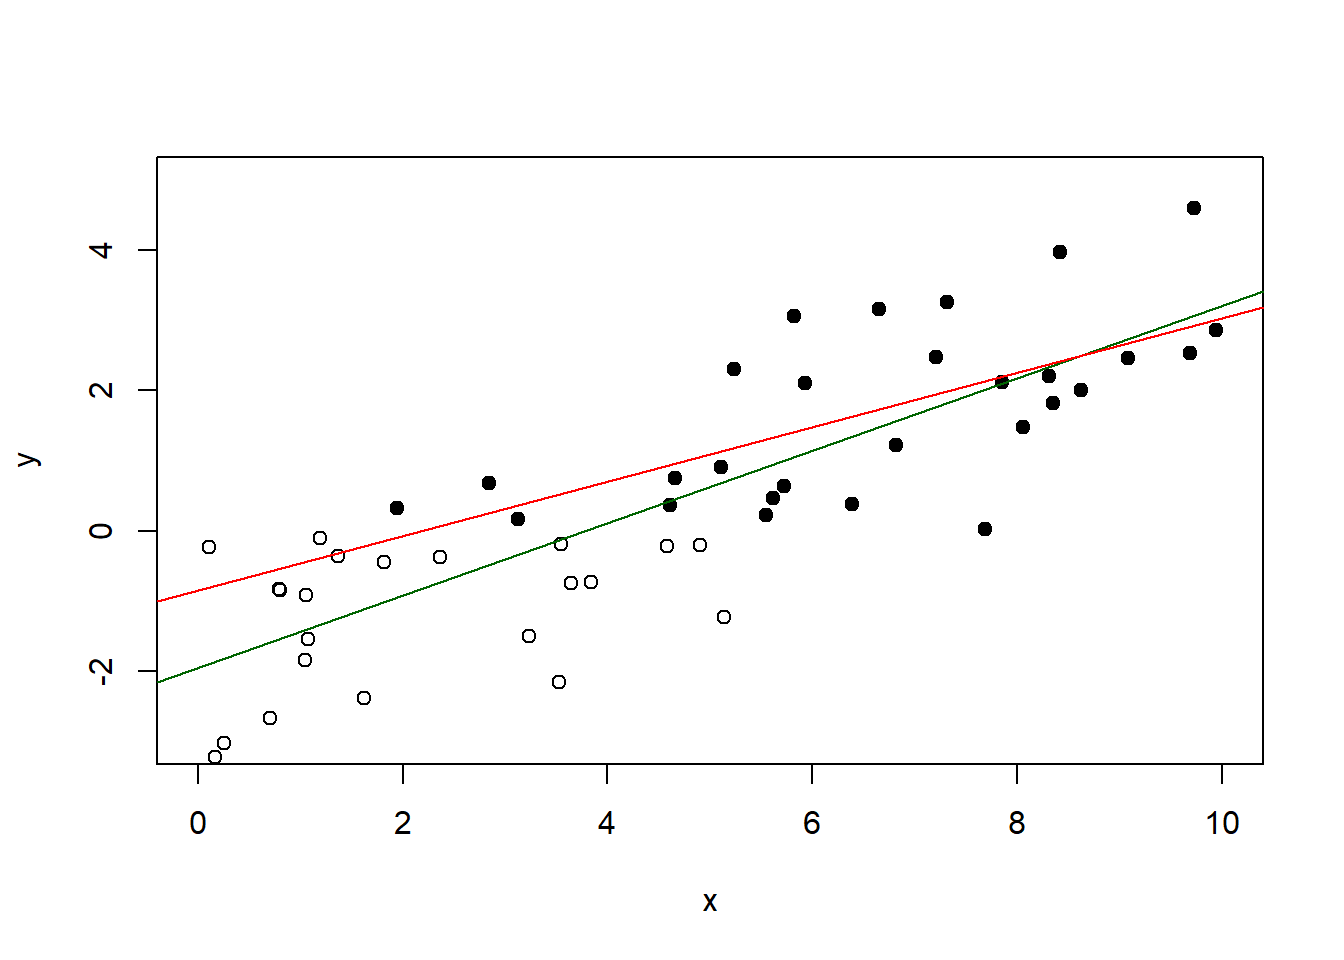
\includegraphics{bookdownproj_files/figure-latex/truncationplot-1.pdf}

If all the data was observed, the correct regression model would give the following results:

\begin{Shaded}
\begin{Highlighting}[]
\KeywordTok{summary}\NormalTok{(bhat_real)}
\end{Highlighting}
\end{Shaded}

\begin{verbatim}
## 
## Call:
## lm(formula = y_real ~ x, data = truncation)
## 
## Residuals:
##      Min       1Q   Median       3Q      Max 
## -1.37440 -0.54465 -0.06085  0.48747  2.43744 
## 
## Coefficients:
##             Estimate Std. Error t value Pr(>|t|)    
## (Intercept) -1.74291    0.24819  -7.022 6.79e-09 ***
## x            0.43954    0.04252  10.338 8.42e-14 ***
## ---
## Signif. codes:  0 '***' 0.001 '**' 0.01 '*' 0.05 '.' 0.1 ' ' 1
## 
## Residual standard error: 0.8392 on 48 degrees of freedom
## Multiple R-squared:  0.6901, Adjusted R-squared:  0.6836 
## F-statistic: 106.9 on 1 and 48 DF,  p-value: 8.423e-14
\end{verbatim}

The estimates are biased if truncation is ignored:

\begin{Shaded}
\begin{Highlighting}[]
\KeywordTok{summary}\NormalTok{(bhat_truncated)}
\end{Highlighting}
\end{Shaded}

\begin{verbatim}
## 
## Call:
## lm(formula = y_obs ~ x, data = truncation)
## 
## Residuals:
##      Min       1Q   Median       3Q      Max 
## -1.49274 -0.56530 -0.01338  0.54597  2.46456 
## 
## Coefficients:
##             Estimate Std. Error t value Pr(>|t|)    
## (Intercept)  -0.8557     0.5930  -1.443 0.160119    
## x             0.3330     0.0837   3.978 0.000446 ***
## ---
## Signif. codes:  0 '***' 0.001 '**' 0.01 '*' 0.05 '.' 0.1 ' ' 1
## 
## Residual standard error: 0.9567 on 28 degrees of freedom
##   (20 observations deleted due to missingness)
## Multiple R-squared:  0.3611, Adjusted R-squared:  0.3382 
## F-statistic: 15.82 on 1 and 28 DF,  p-value: 0.000446
\end{verbatim}

To correct for the truncation, use the functions from the package \href{https://cran.r-project.org/web/packages/truncreg/index.html}{truncreg} which allows to reduce the bias of the coefficients:

\begin{Shaded}
\begin{Highlighting}[]
\NormalTok{bhat_correct =}\StringTok{ }\KeywordTok{truncreg}\NormalTok{(y_obs}\OperatorTok{~}\NormalTok{x,}\DataTypeTok{data=}\NormalTok{truncation)}
\KeywordTok{summary}\NormalTok{(bhat_correct)}
\end{Highlighting}
\end{Shaded}

\begin{verbatim}
## 
## Call:
## truncreg(formula = y_obs ~ x, data = truncation)
## 
## BFGS maximization method
## 41 iterations, 0h:0m:0s 
## g'(-H)^-1g = 4.1E-07 
##  
## 
## 
## Coefficients :
##             Estimate Std. Error t-value Pr(>|t|)    
## (Intercept) -5.15133    2.71321 -1.8986 0.057615 .  
## x            0.81110    0.30288  2.6779 0.007408 ** 
## sigma        1.28107    0.31405  4.0792 4.52e-05 ***
## ---
## Signif. codes:  0 '***' 0.001 '**' 0.01 '*' 0.05 '.' 0.1 ' ' 1
## 
## Log-Likelihood: -31.548 on 3 Df
\end{verbatim}

\hypertarget{censoring}{%
\subsection{Censoring}\label{censoring}}

\begin{Shaded}
\begin{Highlighting}[]
\NormalTok{bhat_real =}\StringTok{ }\KeywordTok{lm}\NormalTok{(y_real}\OperatorTok{~}\NormalTok{x,}\DataTypeTok{data=}\NormalTok{censoring)}
\NormalTok{bhat_censored =}\StringTok{ }\KeywordTok{lm}\NormalTok{(y_obs}\OperatorTok{~}\NormalTok{x,}\DataTypeTok{data=}\NormalTok{censoring)}
\KeywordTok{plot}\NormalTok{(censoring}\OperatorTok{$}\NormalTok{x,censoring}\OperatorTok{$}\NormalTok{y_real)}
     \KeywordTok{points}\NormalTok{(censoring}\OperatorTok{$}\NormalTok{x,censoring}\OperatorTok{$}\NormalTok{y_obs,}\DataTypeTok{pch=}\DecValTok{19}\NormalTok{)}
     \KeywordTok{abline}\NormalTok{(bhat_real)}
     \KeywordTok{abline}\NormalTok{(bhat_censored)}
\end{Highlighting}
\end{Shaded}

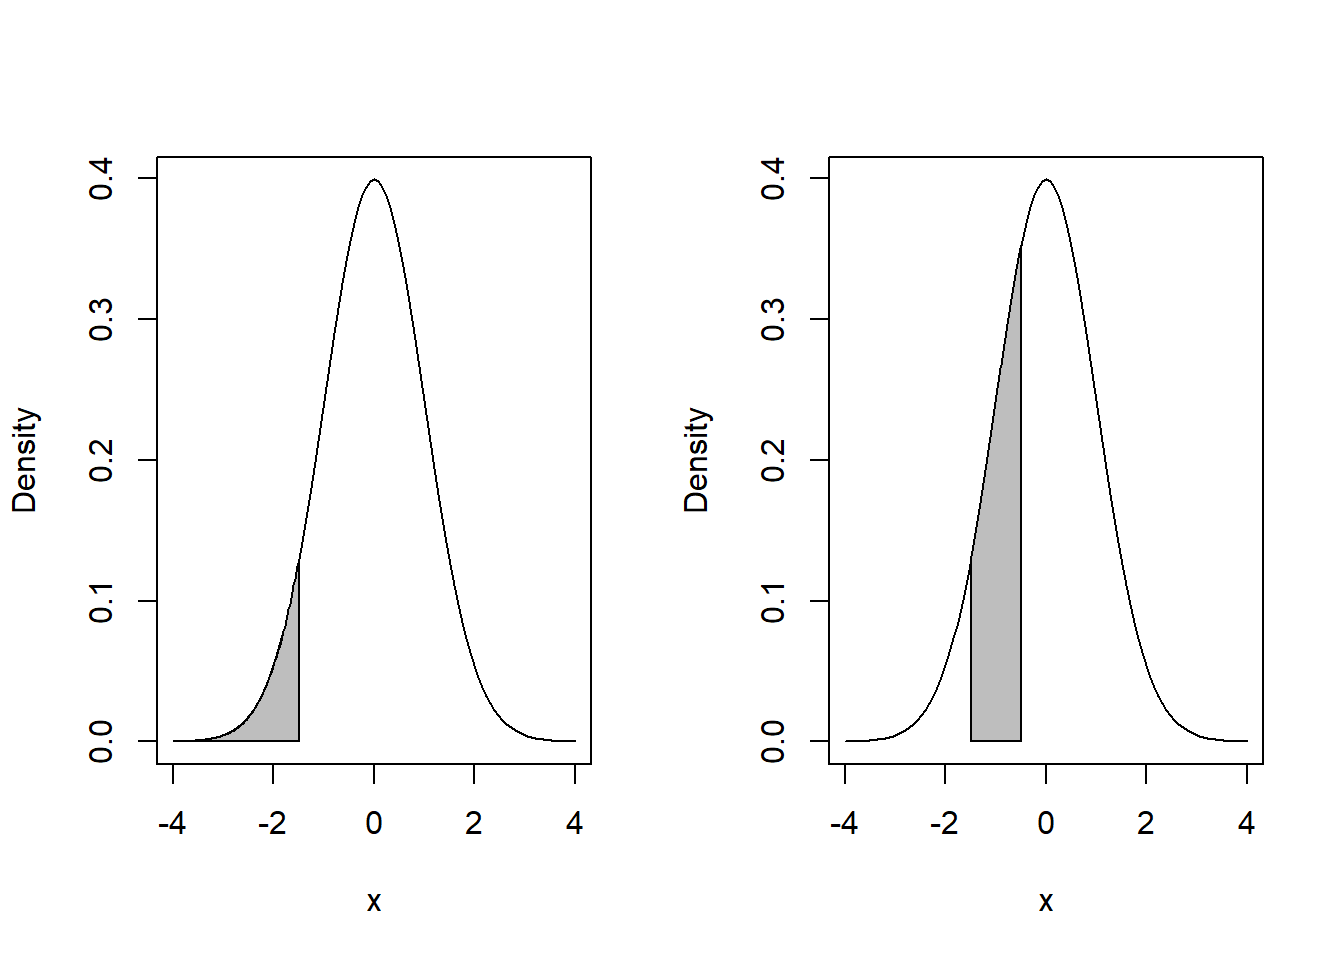
\includegraphics{bookdownproj_files/figure-latex/unnamed-chunk-26-1.pdf}

If all data was reported at the correct value, the following following regression model could be executed:

\begin{Shaded}
\begin{Highlighting}[]
\KeywordTok{summary}\NormalTok{(bhat_real)}
\end{Highlighting}
\end{Shaded}

\begin{verbatim}
## 
## Call:
## lm(formula = y_real ~ x, data = censoring)
## 
## Residuals:
##     Min      1Q  Median      3Q     Max 
## -2.2099 -0.6466 -0.1001  0.7462  2.0724 
## 
## Coefficients:
##             Estimate Std. Error t value Pr(>|t|)    
## (Intercept) -1.79532    0.28614  -6.274 9.54e-08 ***
## x            0.50228    0.05626   8.927 9.07e-12 ***
## ---
## Signif. codes:  0 '***' 0.001 '**' 0.01 '*' 0.05 '.' 0.1 ' ' 1
## 
## Residual standard error: 1.072 on 48 degrees of freedom
## Multiple R-squared:  0.6241, Adjusted R-squared:  0.6163 
## F-statistic:  79.7 on 1 and 48 DF,  p-value: 9.072e-12
\end{verbatim}

Ignoring censoring leads to biased results:

\begin{Shaded}
\begin{Highlighting}[]
\KeywordTok{summary}\NormalTok{(bhat_censored)}
\end{Highlighting}
\end{Shaded}

\begin{verbatim}
## 
## Call:
## lm(formula = y_obs ~ x, data = censoring)
## 
## Residuals:
##     Min      1Q  Median      3Q     Max 
## -1.3968 -0.5504 -0.2154  0.4091  2.2734 
## 
## Coefficients:
##             Estimate Std. Error t value Pr(>|t|)    
## (Intercept) -0.46104    0.20561  -2.242   0.0296 *  
## x            0.30950    0.04043   7.656 7.33e-10 ***
## ---
## Signif. codes:  0 '***' 0.001 '**' 0.01 '*' 0.05 '.' 0.1 ' ' 1
## 
## Residual standard error: 0.7705 on 48 degrees of freedom
## Multiple R-squared:  0.5497, Adjusted R-squared:  0.5404 
## F-statistic: 58.61 on 1 and 48 DF,  p-value: 7.33e-10
\end{verbatim}

Using the R package \href{https://cran.r-project.org/web/packages/censReg/index.html}{censReg}) allows for the reduction of the bias:

\begin{Shaded}
\begin{Highlighting}[]
\NormalTok{b_correct =}\StringTok{ }\KeywordTok{censReg}\NormalTok{(y_obs}\OperatorTok{~}\NormalTok{x,}\DataTypeTok{data=}\NormalTok{censoring)}
\KeywordTok{summary}\NormalTok{(b_correct)}
\end{Highlighting}
\end{Shaded}

\begin{verbatim}
## 
## Call:
## censReg(formula = y_obs ~ x, data = censoring)
## 
## Observations:
##          Total  Left-censored     Uncensored Right-censored 
##             50             22             28              0 
## 
## Coefficients:
##             Estimate Std. error t value  Pr(> t)    
## (Intercept) -1.68234    0.41124  -4.091 4.30e-05 ***
## x            0.47623    0.07031   6.774 1.26e-11 ***
## logSigma     0.06203    0.14026   0.442    0.658    
## ---
## Signif. codes:  0 '***' 0.001 '**' 0.01 '*' 0.05 '.' 0.1 ' ' 1
## 
## Newton-Raphson maximisation, 6 iterations
## Return code 1: gradient close to zero (gradtol)
## Log-likelihood: -52.86668 on 3 Df
\end{verbatim}

\hypertarget{count-regression-models}{%
\subsection{Count Regression Models}\label{count-regression-models}}

Count regression models apply to cases for which the dependent variable represents discrete, integer count data. The main package used is \href{https://cran.r-project.org/web/packages/pscl/index.html}{pscl}. There is also an additional resource with more theoretical details on the topic: \href{http://dx.doi.org/10.18637/jss.v027.i08}{Regression Models for Count Data in R}. A more up-to-date version of the document may be found with the \href{https://cran.r-project.org/web/packages/pscl/index.html}{pscl} package documentation. Here are some examples of count outcomes:

\begin{itemize}
\tightlist
\item
  What are the number of arrests for a person?
\item
  What determines the number of credit cards a person owns?
\end{itemize}

This section on count regression presents three models:

\begin{enumerate}
\def\labelenumi{\arabic{enumi}.}
\item
  Poisson Regression: A condition to use this model is the absence of over- or underdispersion, i.e., the expected value of the dependent variable must be equal to the variance.
\item
  Negative Binomial Regression
\item
\end{enumerate}

\hypertarget{poisson-regression-model}{%
\subsubsection{Poisson Regression Model}\label{poisson-regression-model}}

Recall that the Poisson distribution is written as:
\[Pr(Y=k)=\frac{e^{-\lambda} \cdot \lambda^k}{k!}\]
The important characteristics of the distribution is that the mean and variance are equal to \(\lambda\), i.e., \(E(Y)=\lambda\) and \(Var(Y)=\lambda\), this is also known as the equidispersion property. The mean parameter is written as \(\lambda=exp(\beta_0+\beta_1 \cdot x_1+ \dots + \beta_k \cdot x_k)\).

The first examples uses the 2017 \href{https://nhts.ornl.gov/}{NHTS} data contained in \texttt{hhpub}. In a first step, the data is prepared for the regression model, i.e., missing or unknown values are eliminated and income is measured in dollar terms:

\begin{Shaded}
\begin{Highlighting}[]
\NormalTok{hhpubdata =}\StringTok{ }\KeywordTok{subset}\NormalTok{(hhpub,HHFAMINC }\OperatorTok\StringTok{ }\KeywordTok{c}\NormalTok{(}\DecValTok{1}\OperatorTok{:}\DecValTok{11}\NormalTok{) }\OperatorTok{&}\StringTok{ }\NormalTok{HOMEOWN }\OperatorTok\StringTok{ }\KeywordTok{c}\NormalTok{(}\DecValTok{1}\NormalTok{,}\DecValTok{2}\NormalTok{) }\OperatorTok{&}\StringTok{ }\NormalTok{URBRUR }\OperatorTok\StringTok{ }\KeywordTok{c}\NormalTok{(}\DecValTok{1}\NormalTok{,}\DecValTok{2}\NormalTok{) }\OperatorTok{&}\StringTok{ }\NormalTok{HHVEHCNT }\OperatorTok\StringTok{ }\KeywordTok{c}\NormalTok{(}\DecValTok{1}\OperatorTok{:}\DecValTok{12}\NormalTok{))}
\NormalTok{HHFAMINC =}\StringTok{ }\KeywordTok{c}\NormalTok{(}\DecValTok{1}\OperatorTok{:}\DecValTok{11}\NormalTok{)}
\NormalTok{INCOME =}\StringTok{ }\KeywordTok{c}\NormalTok{(}\DecValTok{10}\NormalTok{,}\FloatTok{12.5}\NormalTok{,}\DecValTok{20}\NormalTok{,}\DecValTok{30}\NormalTok{,}\FloatTok{42.5}\NormalTok{,}\FloatTok{57.5}\NormalTok{,}\FloatTok{82.5}\NormalTok{,}\FloatTok{112.5}\NormalTok{,}\FloatTok{137.5}\NormalTok{,}\DecValTok{175}\NormalTok{,}\DecValTok{200}\NormalTok{)}
\NormalTok{INCOME =}\StringTok{ }\KeywordTok{data.frame}\NormalTok{(HHFAMINC,INCOME)}
\NormalTok{hhpubdata =}\StringTok{ }\KeywordTok{merge}\NormalTok{(hhpubdata,INCOME)}
\NormalTok{hhpubdata}\OperatorTok{$}\NormalTok{RURAL =}\StringTok{ }\NormalTok{hhpubdata}\OperatorTok{$}\NormalTok{URBRUR}\DecValTok{-1}
\NormalTok{hhpubdata}\OperatorTok{$}\NormalTok{RENT =}\StringTok{ }\NormalTok{hhpubdata}\OperatorTok{$}\NormalTok{HOMEOWN}\DecValTok{-1}
\end{Highlighting}
\end{Shaded}

The outcome of interest is the number of vehicles based on household income, home ownership, and urban/rural household location. Before executing the Poisson regression model, calculate the mean and variance of the outcome variable.

\begin{verbatim}
## [1] 1.974733
\end{verbatim}

\begin{verbatim}
## [1] 1.387272
\end{verbatim}

\begin{Shaded}
\begin{Highlighting}[]
\NormalTok{bhat_pois =}\StringTok{ }\KeywordTok{glm}\NormalTok{(HHVEHCNT}\OperatorTok{~}\NormalTok{INCOME}\OperatorTok{+}\NormalTok{RENT}\OperatorTok{+}\NormalTok{RURAL,}\DataTypeTok{data=}\NormalTok{hhpubdata,}\DataTypeTok{family=}\NormalTok{poisson)}
\KeywordTok{summary}\NormalTok{(bhat_pois)}
\end{Highlighting}
\end{Shaded}

\begin{verbatim}
## 
## Call:
## glm(formula = HHVEHCNT ~ INCOME + RENT + RURAL, family = poisson, 
##     data = hhpubdata)
## 
## Deviance Residuals: 
##     Min       1Q   Median       3Q      Max  
## -1.5637  -0.5173  -0.1681   0.2847   5.2201  
## 
## Coefficients:
##               Estimate Std. Error z value Pr(>|z|)    
## (Intercept)  5.163e-01  4.295e-03  120.20   <2e-16 ***
## INCOME       2.608e-03  3.632e-05   71.82   <2e-16 ***
## RENT        -2.466e-01  5.757e-03  -42.84   <2e-16 ***
## RURAL        2.049e-01  4.611e-03   44.44   <2e-16 ***
## ---
## Signif. codes:  0 '***' 0.001 '**' 0.01 '*' 0.05 '.' 0.1 ' ' 1
## 
## (Dispersion parameter for poisson family taken to be 1)
## 
##     Null deviance: 62801  on 118559  degrees of freedom
## Residual deviance: 51828  on 118556  degrees of freedom
## AIC: 353456
## 
## Number of Fisher Scoring iterations: 4
\end{verbatim}

The coefficient estimates are interpreted as follows:

\begin{itemize}
\item
  \(\exp(\beta)\) = with every unit increase in \(X\), the predictor variable has multiplicative effect of \(\exp(\beta)\) on the mean of \(Y\), i.e., \(\lambda\)
\item
  If \(\beta=0\), then \(\exp(\beta) = 1\), and the expected count \(\mu= E(y) = \exp(\alpha)\), and Y and X are not related.
\item
  If \(\beta>0\), then \(\exp(\beta) > 1\), and the expected count \(E(y)\) is \(\exp(\beta)\) times larger than when \(X = 0\)
\item
  If \(\beta<0\), then \(\exp(\beta) < 1\), and the expected count \(E(y)\) is \(\exp(\beta)\) times smaller than when \(X = 0\)
\end{itemize}

To estimate a negative binomial model:

\begin{Shaded}
\begin{Highlighting}[]
\NormalTok{bhat_nb =}\StringTok{ }\KeywordTok{glm}\NormalTok{(HHVEHCNT}\OperatorTok{~}\NormalTok{INCOME}\OperatorTok{+}\NormalTok{RENT}\OperatorTok{+}\NormalTok{RURAL,}\DataTypeTok{data=}\NormalTok{hhpubdata)}
\KeywordTok{summary}\NormalTok{(bhat_nb)}
\end{Highlighting}
\end{Shaded}

\begin{verbatim}
## 
## Call:
## glm(formula = HHVEHCNT ~ INCOME + RENT + RURAL, data = hhpubdata)
## 
## Deviance Residuals: 
##     Min       1Q   Median       3Q      Max  
## -2.2407  -0.7306  -0.2535   0.4696  10.3238  
## 
## Coefficients:
##               Estimate Std. Error t value Pr(>|t|)    
## (Intercept)  1.622e+00  6.263e-03  259.00   <2e-16 ***
## INCOME       5.830e-03  5.735e-05  101.66   <2e-16 ***
## RENT        -4.270e-01  7.656e-03  -55.77   <2e-16 ***
## RURAL        4.525e-01  7.212e-03   62.75   <2e-16 ***
## ---
## Signif. codes:  0 '***' 0.001 '**' 0.01 '*' 0.05 '.' 0.1 ' ' 1
## 
## (Dispersion parameter for gaussian family taken to be 1.058507)
## 
##     Null deviance: 148367  on 118559  degrees of freedom
## Residual deviance: 125492  on 118556  degrees of freedom
## AIC: 343206
## 
## Number of Fisher Scoring iterations: 2
\end{verbatim}

\hypertarget{negative-binomial-model}{%
\subsubsection{Negative-Binomial Model}\label{negative-binomial-model}}

MODEL 1: Basic model of resource mobilization and opportunity structure

\begin{Shaded}
\begin{Highlighting}[]
\NormalTok{nb}\FloatTok{.3}\NormalTok{_}\DecValTok{1}\NormalTok{ =}\StringTok{ }\KeywordTok{glm.nb}\NormalTok{(tot.protests }\OperatorTok{~}\StringTok{ }\KeywordTok{log}\NormalTok{(TotalPop) }\OperatorTok{+}\StringTok{ }\KeywordTok{log}\NormalTok{(pop.density) }\OperatorTok{+}\StringTok{ }\NormalTok{Per_Black }\OperatorTok{+}\StringTok{ }\NormalTok{BlackPovertyRate }\OperatorTok{+}\StringTok{ }\KeywordTok{I}\NormalTok{(BlackPovertyRate}\OperatorTok{^}\DecValTok{2}\NormalTok{) }\OperatorTok{+}\StringTok{ }\NormalTok{per_ba }\OperatorTok{+}\StringTok{ }\NormalTok{collegeenrollpc }\OperatorTok{+}\StringTok{ }\NormalTok{dem_share , }\DataTypeTok{data=}\NormalTok{blm, }\DataTypeTok{link=}\NormalTok{log)}
\KeywordTok{summary}\NormalTok{(nb}\FloatTok{.3}\NormalTok{_}\DecValTok{1}\NormalTok{) }
\end{Highlighting}
\end{Shaded}

\begin{verbatim}
## 
## Call:
## glm.nb(formula = tot.protests ~ log(TotalPop) + log(pop.density) + 
##     Per_Black + BlackPovertyRate + I(BlackPovertyRate^2) + per_ba + 
##     collegeenrollpc + dem_share, data = blm, link = log, init.theta = 1.559078735)
## 
## Deviance Residuals: 
##     Min       1Q   Median       3Q      Max  
## -2.2523  -0.4543  -0.2673  -0.1506   5.7386  
## 
## Coefficients:
##                         Estimate Std. Error z value Pr(>|z|)    
## (Intercept)           -2.090e+01  1.117e+00 -18.719  < 2e-16 ***
## log(TotalPop)          1.292e+00  7.159e-02  18.047  < 2e-16 ***
## log(pop.density)      -3.130e-01  1.328e-01  -2.356  0.01848 *  
## Per_Black              2.249e-02  4.709e-03   4.777 1.78e-06 ***
## BlackPovertyRate       1.319e-01  3.121e-02   4.227 2.37e-05 ***
## I(BlackPovertyRate^2) -1.340e-03  4.768e-04  -2.810  0.00496 ** 
## per_ba                 4.462e-02  5.465e-03   8.163 3.26e-16 ***
## collegeenrollpc        1.051e-02  4.118e-03   2.553  0.01068 *  
## dem_share              4.077e-02  7.292e-03   5.591 2.26e-08 ***
## ---
## Signif. codes:  0 '***' 0.001 '**' 0.01 '*' 0.05 '.' 0.1 ' ' 1
## 
## (Dispersion parameter for Negative Binomial(1.5591) family taken to be 1)
## 
##     Null deviance: 1899.84  on 1225  degrees of freedom
## Residual deviance:  501.15  on 1217  degrees of freedom
##   (133 observations deleted due to missingness)
## AIC: 1120.2
## 
## Number of Fisher Scoring iterations: 1
## 
## 
##               Theta:  1.559 
##           Std. Err.:  0.351 
## 
##  2 x log-likelihood:  -1100.187
\end{verbatim}

\begin{Shaded}
\begin{Highlighting}[]
\CommentTok{# MODEL 2: Adding black deaths}
\NormalTok{nb}\FloatTok{.3}\NormalTok{_}\DecValTok{2}\NormalTok{ <-}\StringTok{ }\KeywordTok{glm.nb}\NormalTok{(tot.protests }\OperatorTok{~}\StringTok{ }\KeywordTok{log}\NormalTok{(TotalPop) }\OperatorTok{+}\StringTok{ }\KeywordTok{log}\NormalTok{(pop.density) }\OperatorTok{+}\StringTok{ }\NormalTok{Per_Black }\OperatorTok{+}\StringTok{ }\NormalTok{BlackPovertyRate }\OperatorTok{+}\StringTok{ }\KeywordTok{I}\NormalTok{(BlackPovertyRate}\OperatorTok{^}\DecValTok{2}\NormalTok{) }\OperatorTok{+}\StringTok{ }\NormalTok{per_ba }\OperatorTok{+}\StringTok{ }\NormalTok{collegeenrollpc }\OperatorTok{+}\StringTok{ }\NormalTok{dem_share }\OperatorTok{+}\StringTok{ }\NormalTok{deaths_black_pc, }\DataTypeTok{data=}\NormalTok{blm, }\DataTypeTok{link=}\NormalTok{log)}
\KeywordTok{summary}\NormalTok{(nb}\FloatTok{.3}\NormalTok{_}\DecValTok{2}\NormalTok{) }
\end{Highlighting}
\end{Shaded}

\begin{verbatim}
## 
## Call:
## glm.nb(formula = tot.protests ~ log(TotalPop) + log(pop.density) + 
##     Per_Black + BlackPovertyRate + I(BlackPovertyRate^2) + per_ba + 
##     collegeenrollpc + dem_share + deaths_black_pc, data = blm, 
##     link = log, init.theta = 1.685551835)
## 
## Deviance Residuals: 
##     Min       1Q   Median       3Q      Max  
## -2.3170  -0.4549  -0.2707  -0.1529   5.3090  
## 
## Coefficients:
##                         Estimate Std. Error z value Pr(>|z|)    
## (Intercept)           -2.073e+01  1.101e+00 -18.824  < 2e-16 ***
## log(TotalPop)          1.281e+00  7.046e-02  18.178  < 2e-16 ***
## log(pop.density)      -3.054e-01  1.315e-01  -2.323 0.020201 *  
## Per_Black              1.801e-02  4.864e-03   3.704 0.000212 ***
## BlackPovertyRate       1.283e-01  3.109e-02   4.127 3.67e-05 ***
## I(BlackPovertyRate^2) -1.301e-03  4.743e-04  -2.744 0.006071 ** 
## per_ba                 4.372e-02  5.381e-03   8.125 4.47e-16 ***
## collegeenrollpc        1.005e-02  4.073e-03   2.466 0.013657 *  
## dem_share              4.069e-02  7.249e-03   5.613 1.98e-08 ***
## deaths_black_pc        2.825e+00  9.312e-01   3.034 0.002414 ** 
## ---
## Signif. codes:  0 '***' 0.001 '**' 0.01 '*' 0.05 '.' 0.1 ' ' 1
## 
## (Dispersion parameter for Negative Binomial(1.6856) family taken to be 1)
## 
##     Null deviance: 1943.21  on 1225  degrees of freedom
## Residual deviance:  500.18  on 1216  degrees of freedom
##   (133 observations deleted due to missingness)
## AIC: 1113.4
## 
## Number of Fisher Scoring iterations: 1
## 
## 
##               Theta:  1.686 
##           Std. Err.:  0.404 
## 
##  2 x log-likelihood:  -1091.353
\end{verbatim}

\begin{Shaded}
\begin{Highlighting}[]
\CommentTok{# MODEL 3: Using all police-caused deaths instead (victims of any race)}
\NormalTok{nb}\FloatTok{.3}\NormalTok{_}\DecValTok{3}\NormalTok{ <-}\StringTok{ }\KeywordTok{glm.nb}\NormalTok{(tot.protests }\OperatorTok{~}\StringTok{ }\KeywordTok{log}\NormalTok{(TotalPop) }\OperatorTok{+}\StringTok{ }\KeywordTok{log}\NormalTok{(pop.density) }\OperatorTok{+}\StringTok{ }\NormalTok{Per_Black }\OperatorTok{+}\StringTok{ }\NormalTok{BlackPovertyRate }\OperatorTok{+}\StringTok{ }\KeywordTok{I}\NormalTok{(BlackPovertyRate}\OperatorTok{^}\DecValTok{2}\NormalTok{) }\OperatorTok{+}\StringTok{ }\NormalTok{per_ba }\OperatorTok{+}\StringTok{ }\NormalTok{collegeenrollpc }\OperatorTok{+}\StringTok{ }\NormalTok{dem_share }\OperatorTok{+}\StringTok{ }\NormalTok{deaths_pc, }\DataTypeTok{data=}\NormalTok{blm, }\DataTypeTok{link=}\NormalTok{log)}
\KeywordTok{summary}\NormalTok{(nb}\FloatTok{.3}\NormalTok{_}\DecValTok{3}\NormalTok{) }
\end{Highlighting}
\end{Shaded}

\begin{verbatim}
## 
## Call:
## glm.nb(formula = tot.protests ~ log(TotalPop) + log(pop.density) + 
##     Per_Black + BlackPovertyRate + I(BlackPovertyRate^2) + per_ba + 
##     collegeenrollpc + dem_share + deaths_pc, data = blm, link = log, 
##     init.theta = 1.621799986)
## 
## Deviance Residuals: 
##     Min       1Q   Median       3Q      Max  
## -2.3230  -0.4517  -0.2684  -0.1505   5.6311  
## 
## Coefficients:
##                         Estimate Std. Error z value Pr(>|z|)    
## (Intercept)           -2.080e+01  1.108e+00 -18.773  < 2e-16 ***
## log(TotalPop)          1.277e+00  7.122e-02  17.928  < 2e-16 ***
## log(pop.density)      -3.121e-01  1.321e-01  -2.363  0.01812 *  
## Per_Black              2.163e-02  4.705e-03   4.596 4.31e-06 ***
## BlackPovertyRate       1.295e-01  3.110e-02   4.164 3.12e-05 ***
## I(BlackPovertyRate^2) -1.315e-03  4.744e-04  -2.772  0.00558 ** 
## per_ba                 4.507e-02  5.472e-03   8.237  < 2e-16 ***
## collegeenrollpc        1.040e-02  4.094e-03   2.540  0.01108 *  
## dem_share              4.121e-02  7.257e-03   5.678 1.36e-08 ***
## deaths_pc              9.564e-01  6.330e-01   1.511  0.13085    
## ---
## Signif. codes:  0 '***' 0.001 '**' 0.01 '*' 0.05 '.' 0.1 ' ' 1
## 
## (Dispersion parameter for Negative Binomial(1.6218) family taken to be 1)
## 
##     Null deviance: 1921.82  on 1225  degrees of freedom
## Residual deviance:  502.82  on 1216  degrees of freedom
##   (133 observations deleted due to missingness)
## AIC: 1119.8
## 
## Number of Fisher Scoring iterations: 1
## 
## 
##               Theta:  1.622 
##           Std. Err.:  0.374 
## 
##  2 x log-likelihood:  -1097.839
\end{verbatim}

\hypertarget{data-sources}{%
\section{Data Sources}\label{data-sources}}

This chapter describes the data sets associated with these lecture notes. Some data sets are generic, i.e., randomly generated, to highlight a particular concept while other are either based on public sources or are taken from academic papers. In any case, the source is clearly indicated. Sometimes modifications were made to the data sets for ease of use, e.g., removing missing values. All the data are contained in the file \href{https://github.com/jrfdumortier/dataanalysis/blob/master/DataAnalysisPAData.RData}{DataAnalysisPAData.RData}.

\begin{itemize}
\item
  \texttt{accidents} (\(N=30\)): Generic data on the number of accidents (\emph{accidents}) and the temperature in Fahrenheit (\emph{temperature}).
\item
  \texttt{airlines} (\(N=189496\)): Data on airline on-time statistics and delay causes from the Bureau of Transportation Statistics from January 2004 to May 2020. The variable names are mostly self-explanatory. The variables \emph{arr\_flights} and \emph{arr\_del15} are the total number of arrival flights and the number of flight delayed at least 15 minutes. The original dataset is available \href{https://www.transtats.bts.gov/ot_delay/ot_delaycause1.asp}{here}.
\item
  \texttt{anscombe} (\(N=11\)): Anscombe's Quartet where \(y_i\) and \(x_1\) represent dependent and independent variable of set \(i\), respectively.
\item
  \texttt{bmw} (\(N=30\)): Data on the prices and miles of a particular BMW 5 series model in the Indianapolis area. Some of the models have rear-wheel drive whereas some have all-wheel drive (\(allwheeldrive=1\)).
\item
  \texttt{coffee} (\(N=29\)): Historical data about the coffee consumption in the United States. The variable \emph{consumption} is measured in thousand 60-kg bags. The variable \emph{price} represents the retail price of roasted coffee in US Dollars per pound. Both time series are obtained from the International Coffee Association. The variables \emph{rdi} and \emph{cpi} represent real disposable income and the consumer price index, respectively. Those data series are obtained from the St.~Louis FRED date base. The same is true for the varible \emph{population}. The variables \emph{rprice} and \emph{pcconsumption} represent the real coffee prices and the per-capita consumption of coffee.
\item
  \texttt{compactcars} (\(N=78\)): Fuel efficiency of compact cars in 1995 and 2015. The fuel efficiceny is expressed in miles per gallon in the columns \emph{Automatic} and \emph{Manual}, respectively.
\item
  \texttt{discharge} (\(N=7\)): Generic data set of pollutant discharge into a river measured in gallons.
\item
  \texttt{eggweights} (\(N=37\)): Weight in grams of Large Grade A Brown Eggs from Whole Foods.
\item
  \texttt{eucrime} (\(N=387\)): Intentional homicide data in Europe. Data series \texttt{crim\_hom\_soff} from Eurostat.
\item
  \texttt{evdata} (\(N=579\)): Data about the choice of consumers with respect to alternative fuel vehicles. The
  variable \emph{choice} represents the choice by the consumer for gasoline vehicles (\(choice = 1\)), conventional
  hybrids (\(choice = 2\)), plug-in hybrids (\(choice = 3\)), and electric vehicles (\(choice = 4\)). For each consumer,
  you have the following variables: \emph{age}, \emph{level2} (indicating whether people have a fast charger for electric cars in their community), \emph{female}, and \emph{numcars} (number of cars). The variable \emph{politics} is coded as follows: Under \$15,000 (1), \$15,000 to \$24,999 (2), \$25,000 to \$34, 999 (3), \$35,000 to \$49,999 (4), \$50,000 to \$74,999 (5), \$75,000 to \$99,999 (6), \$100,000 to \$149,999 (7), \$150,000 to \$199,999 (8), \$200,000 to \$249,000 (9), above \$250,000 (10). The variable \emph{edu} is coded as follows: Less than High School (1), High School / GED (2), Some College (3), 2-year College Degree (4), 4-year College Degree (5), Masters Degree (6), Doctoral Degree (7). The variable politics is coded as follows: Extremely Liberal (1), Liberal (2), Slightly liberal (3), Moderate (4), Slightly conservative (5), Conservative (6), Extremely conservative (7), Other (8), None (9). See \citet{Dumortier:2014} for more details.
\item
  \texttt{fpdata} (\(N=176\)):
\item
  \texttt{gss2018} (\(N=772\)): 2018 data from the General Social Survey with the followin variables:

  \begin{itemize}
          \item \emph{fulltime}: Working full time (dummy variable $yes=1$)
          \item \emph{government}: Working for the government ($yes=1$)
          \item \emph{married}: Being married ($yes=1$) 
          \item \emph{education}: Highest degree from high school (1), junior college (2),  bachelor (3), graduate (4). 
          \item \emph{age}: Age of the respondent.
          \item \emph{childs}:
          \item \emph{vote}: Voted in the 2016 election ($yes=1$).
          \item \emph{income}: Income of the respondent taking as the average over the range from the GSS.
          \item \emph{gun}: Gun ownership ($yes=1$).
          \item \emph{deathpenalty}: Favoring the death penalty ($yes=1$).
          \item \emph{totalwealth}: Total wealther of the respondent taking as the average over the range from the GSS.
     \end{itemize}
\item
  \texttt{gssgun} (\(N=1300\)):
\item
  \texttt{gsssocialmedia} (\(N=1366\)):
\item
  \texttt{happy} (\(N=631\)): Data from the 2018 General Social Survey about happiness which includes the following variables:

  \begin{itemize}
  \tightlist
  \item
    \(sexfreq\): Frequency of sex during last year
  \item
    \(gun\): Have gun in home
  \item
    \(sclass\): Subjective class identification
  \item
    \(health1\): Condition of health
  \item
    \(happiness\): General happiness
  \item
    \(party\): Political party affiliation. You may want to combine the \texttt{Ind,\ near\ democrat\textquotesingle{}\textquotesingle{}\ and}Not str democrat'' into the same category, e.g., ``lean democrat''. Do the same for republicans.
  \item
    \(education\): Highest year of school completed
  \item
    \(age\): Age of respondent
  \end{itemize}
\item
  \texttt{hdr} (\(N=189\)): Human Development Indicator from 2019.
\item
  \texttt{heating} (\(N=24\)): Contains 24 observations of natural gas usage (in hundreds of cubic feet) and the average outside temperature (in Fahrenheit).
\item
  \texttt{hhpub} (\(N=129696\)):
\item
  \texttt{honda} (\(N=81\)):
\item
  \texttt{hybrid} (\(N=1000\)):
\item
  \texttt{indyhomes} (\(N=102\)):
\item
  \texttt{meatdemand} (\(N=39\)): Meet demand quantity (\(q\)) and real price (\(p\)) data from the U.S. Department of Agriculture. Prices and real disposable income (\(rdi\)) are in real terms.
\item
  \texttt{mh1} (\(N=101\)): Home values in the Meridian Hills area in Indianapolis.
\item
  \texttt{mh2} (\(N=18\)): Prices and characteristics of homes in the Meridian Hills area in Indianapolis.
\item
  \texttt{milk} (\(N=50\)): Randomly generated milk container fillings in ounces.
\item
  \texttt{mpa} (\(N=18\)): Randomly generated exam scores in a class of MPA students.
\item
  \texttt{nfl} (\(N=1009\)): Data from \citet{Berri:2011} which includes the following variables:

  \begin{itemize}
  \item \emph{total}: Total salary
  \item \emph{yards}: Passing yards from the prior season
  \item \emph{att}: Pass attempts
  \item \emph{exp}: Total years of experience in the league.
  \item \emph{esp2}: Total years of experience in the league squared.
  \item \emph{draft1}: First round draft pick.
  \item \emph{draft2}: Second round draft pick.
  \item \emph{veteran}: Bargaining status changes after a player has completed three years in the NFL.
  \item \emph{changeteam}: Player has changed team.
  \item \emph{pbowlever}: Player appeared in the Pro Bowl.
  \item \emph{symm}: Facial symmetry.
  \end{itemize}
\item
  \texttt{ohioincome} (\(N=607\)): Enrollment and median income in Ohio School districts for 2018/2019. \emph{IRN} identifies the school district.
\item
  \texttt{ohioscore} (\(N=608\)): Performance and achievement scores of Ohio schools for 2018/2019. The data is obtained from the \href{https://reportcard.education.ohio.gov/}{Ohio Department of Education}. \emph{IRN} identifies the school district.
\item
  \texttt{organic} (\(N=100\)): Randomly generated data on the purchase behavior of organic food (binary choice) as a function of income.
\item
  `retail\} (\(N=348\)): \href{https://fred.stlouisfed.org/series/RSXFSN}{Advance Retail Sales: Retail (Excluding Food Services)} obtained from the St; Louis FRED.
\item
  \texttt{skewness} (\(N=500\)): Randomly generated data from a beta distribution:

  \begin{itemize}
  \item \emph{beta55}: $a=5$ and $b=5$.
  \item \emph{beta28}: $a=2$ and $b=8$.
  \item \emph{beta82}: $a=8$ and $b=2$.
  \end{itemize}
\item
  \texttt{soda} (\(N=25\)): Randomly generated data of for soda cans (in milliliters).
\item
  \texttt{states} (\(N=10\)): Generated income data for three states.
\item
  \texttt{usdata} (\(N=296\)): Data from the St.~Louis FRED data base.

  \begin{itemize}
  \item \emph{income}: Real Disposable Personal Income: Per Capita
  \item \emph{consumption}: Real personal consumption expenditures per capita
  \end{itemize}
\item
  \texttt{vehicles} (\(N=42702\)): The data set contains data about the fuel efficiency of vehicles from model year 1984 to 2021 (\(year\)). It also includes \(make\) and \(model\) for the various manufacturers. The variable \(displ\) refers to engine displacement in liters\footnote{\url{https://en.wikipedia.org/wiki/Engine_displacement}}, \(VClass\) is the vehicle class, \(ghgScore\) indicates the greenhouse gas (GHG) emissions, and \(comb08U\) is unrounded combined MPG. The data is obtained from the U.S. Environmental Protection Agency' (EPA) \href{https://www.fueleconomy.gov/feg/download.shtml}{Fuel Economy Data} webpage.
\item
  \texttt{vehpub} (\(N=256115\)): The data contains vehicle data from the 2017 National Household Travel Survey (NHTS). I have deleted some columns but the detailed code book can be found \href{https://nhts.ornl.gov/tables09/CodebookBrowser.aspx}{here}. The variables included are:

  \begin{itemize}
  \item \emph{HOUSEID}: Household Identifier 
  \item \emph{VEHID}: Vehicle Identifier
  \item \emph{VEHYEAR}: Vehicle Year
  \item \emph{MAKE}: Vehicle Make
  \item \emph{FUELTYPE}: Fuel Type
  \item \emph{VEHTYPE}: Vehicle Type
  \item \emph{OD\_READ}: Odometer Reading
  \item \emph{HFUEL}: Type of Hybrid Vehicle
  \item \emph{HYBRID}: Hybrid vehicle
  \item \emph{HOMEOWN}: Home Ownership
  \item \emph{HHFAMINC}: Household income
  \item \emph{HHSTATE}: Household state
  \item \emph{URBRUR}: Household in urban/rural area
  \end{itemize}
\item
  \texttt{waterpressure} (\(N=30\)): Generated data on the water pressure in city's water lines.
\item
  \texttt{wdi} (\(N=13237\)): World Development Indicators (WDI) from the World Bank. The following variables are included in the data set.
\end{itemize}

\textbackslash begin\{itemize\}

\item

\emph{iso2c}: Country code

\item

\emph{country}: Country name

\item

\emph{year}: Year

\item

\emph{gdp}: GDP per capita (constant 2010 US\$)

\item

\emph{lifeexp}: Life expectancy at birth, total (years)

\item

\emph{litrate}: Literacy rate, adult total (\% of people ages 15 and above)

\item

\emph{fertrate}: Fertility rate, total (births per woman)

\item

\emph{mortrate}: Mortality rate, under 5 (per 1,000 live births)

\item

\emph{region}: \href{https://datahelpdesk.worldbank.org/knowledgebase/articles/378834-how-does-the-world-bank-classify-countries}{Geographic regions}

\item

\emph{incomeLevel}: Income groupings are based on Gross National Income per capita

\end{document}
